% THIS IS AN EXAMPLE DOCUMENT FOR VLDB 2010
% based on ACM SIGPROC-SP.TEX VERSION 2.7
% Modified by  Gerald Weber <gerald@cs.auckland.ac.nz>


% This example *does* use the .bib file (from which the .bbl file
% is produced). REMEMBER HOWEVER: After having produced the .bbl file,
% and prior to final submission, you need to 'insert'  your .bbl file into
% your source .tex file so as to provide ONE 'self-contained' source file.


\documentclass[a4paper,12pt]{report}
\renewcommand{\baselinestretch}{1.5}
%\usepackage[linesnumbered,boxed]{algorithm2e}
\usepackage{amsmath}
\usepackage{amsthm}
%\usepackage{algorithm}
\usepackage{algorithmic}
\usepackage[ruled]{algorithm2e}
%\usepackage{algpseudocode}
\usepackage{graphicx}
\usepackage{verbatim}
\usepackage{latexsym}
\usepackage{subfigure}
\usepackage{subfig}
\usepackage{color}

\usepackage{float}
\usepackage{indentfirst}
\usepackage{wallpaper}
\usepackage{pdfpages}
\usepackage{multirow}
\newtheorem{theorem}{Theorem}
%\usepackage{pdfpages}
%\usepackage{hyperref}
\usepackage{CJK}
%let table don't cross another section
\usepackage[section]{placeins}

\CenterWallPaper{.30}{figure/nthu-logo.pdf}

%set paper size
\special{papersize=8.5in,11in}
\topmargin=14.7mm    %bottom margin 14.7mm
\oddsidemargin=30mm   %left & right margin 17.45mm

%text sizes (Keep these values unchanged!)
\textwidth=150mm \textheight=250mm
\columnsep=5.0mm
\parindent=3.5mm

%misc parameters
\headsep=0mm  \headheight=0mm \footskip=18mm

%conversion to values for LaTeX
\advance\topmargin-1in\advance\oddsidemargin-1in
\evensidemargin\oddsidemargin


\begin{document}

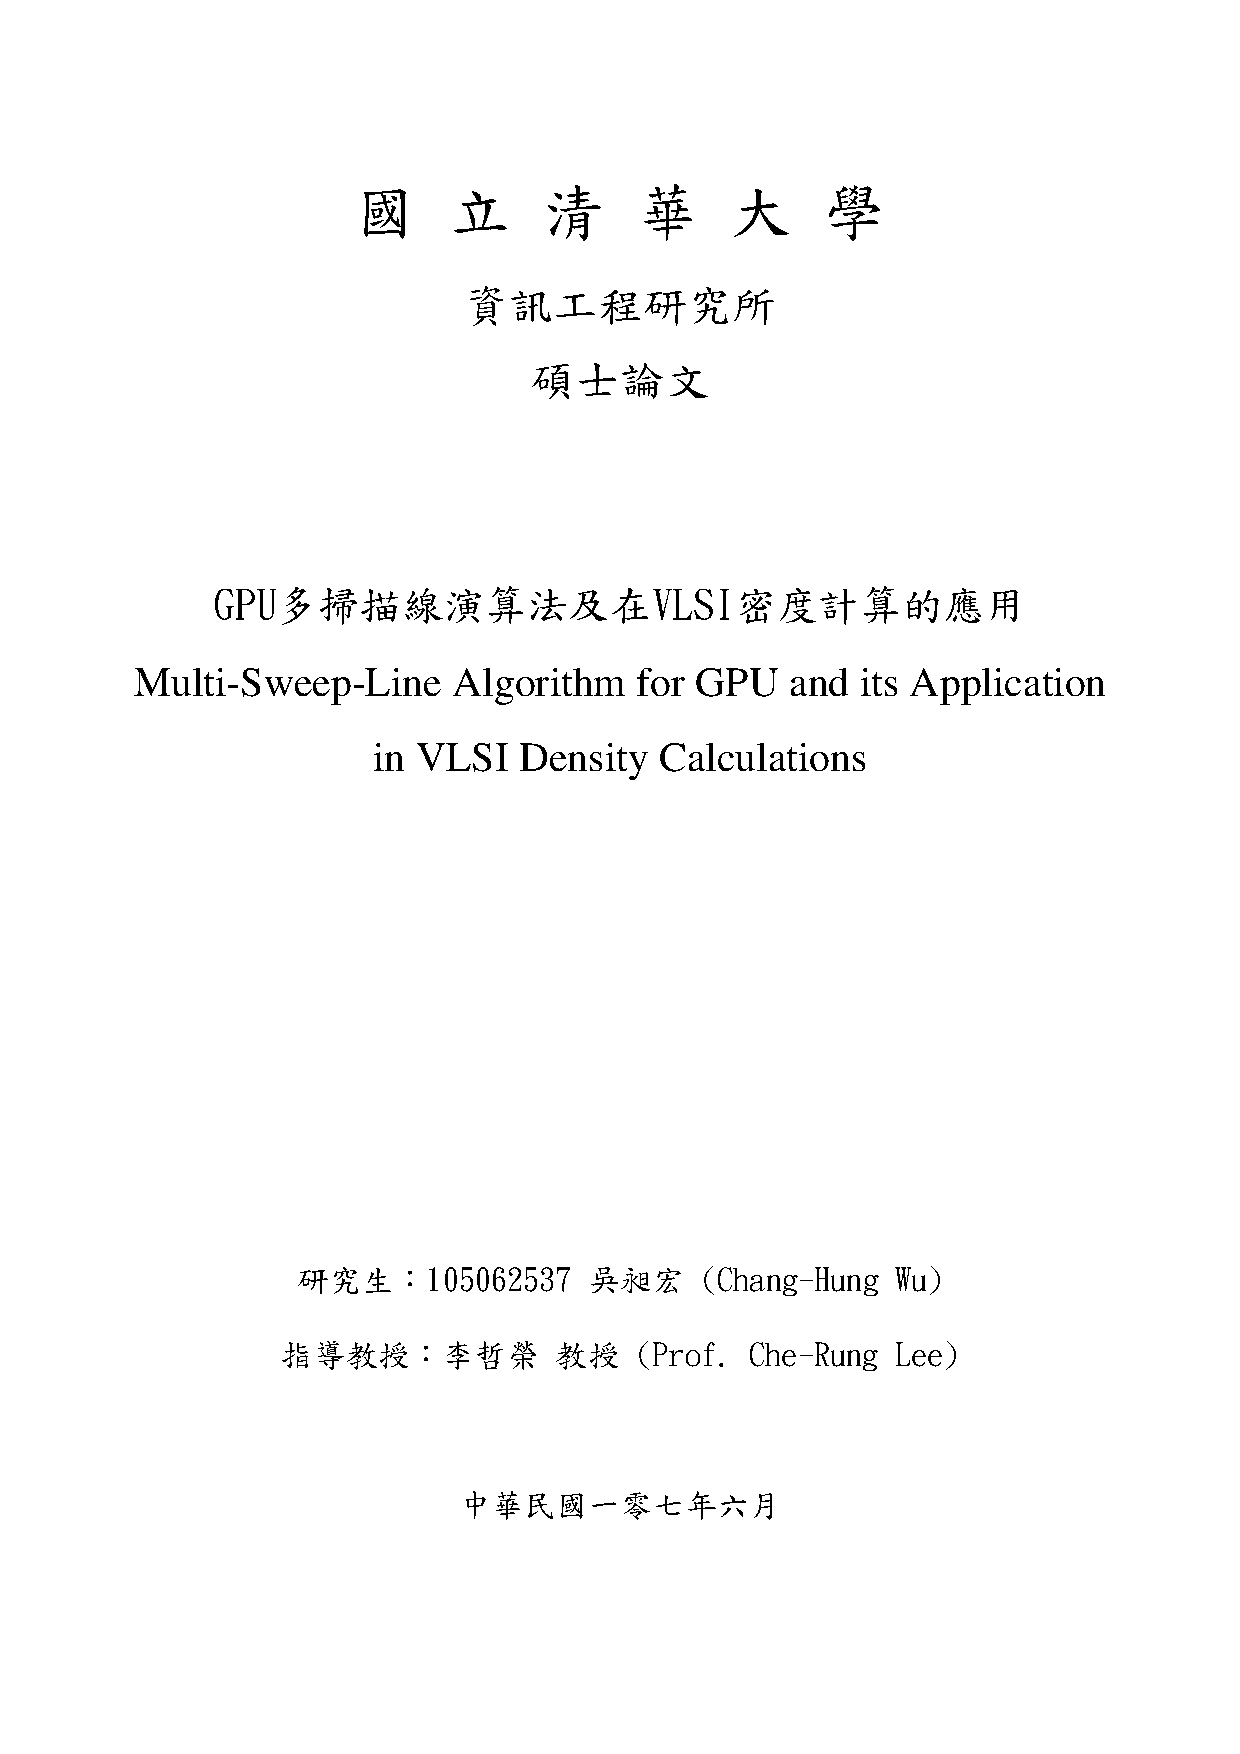
\includepdf[pages={1}]{cover.pdf}
%\includepdf[pages={1}]{cover_ch.pdf}

\title{\bf \huge qCUDA-ARM: A GPGPU Virtualization solution  NVIDIA TX2
}
\date{}
\author{
\begin{tabular}{c}
\\
\\
{\LARGE \bf Student: Bo-Yu Huang}\\
{\LARGE \bf Advisor: Prof. Che-Rung Lee}\\
\\
\\
\\
\\
{\LARGE \bf Department of Computer Science}\\
{\LARGE \bf National Tsing Hua University}\\
{\LARGE \bf Hsinchu, Taiwan, 30013, R.O.C.}\\
\\
{\large June 2019}
\end{tabular}
}

\maketitle
\includepdfset{pagecommand={\thispagestyle{plain}}}

\pagenumbering{roman}
%\addcontentsline{toc}{chapter}{\ctxfr 中文摘要}
\addcontentsline{toc}{chapter}{Chinese Abstract}
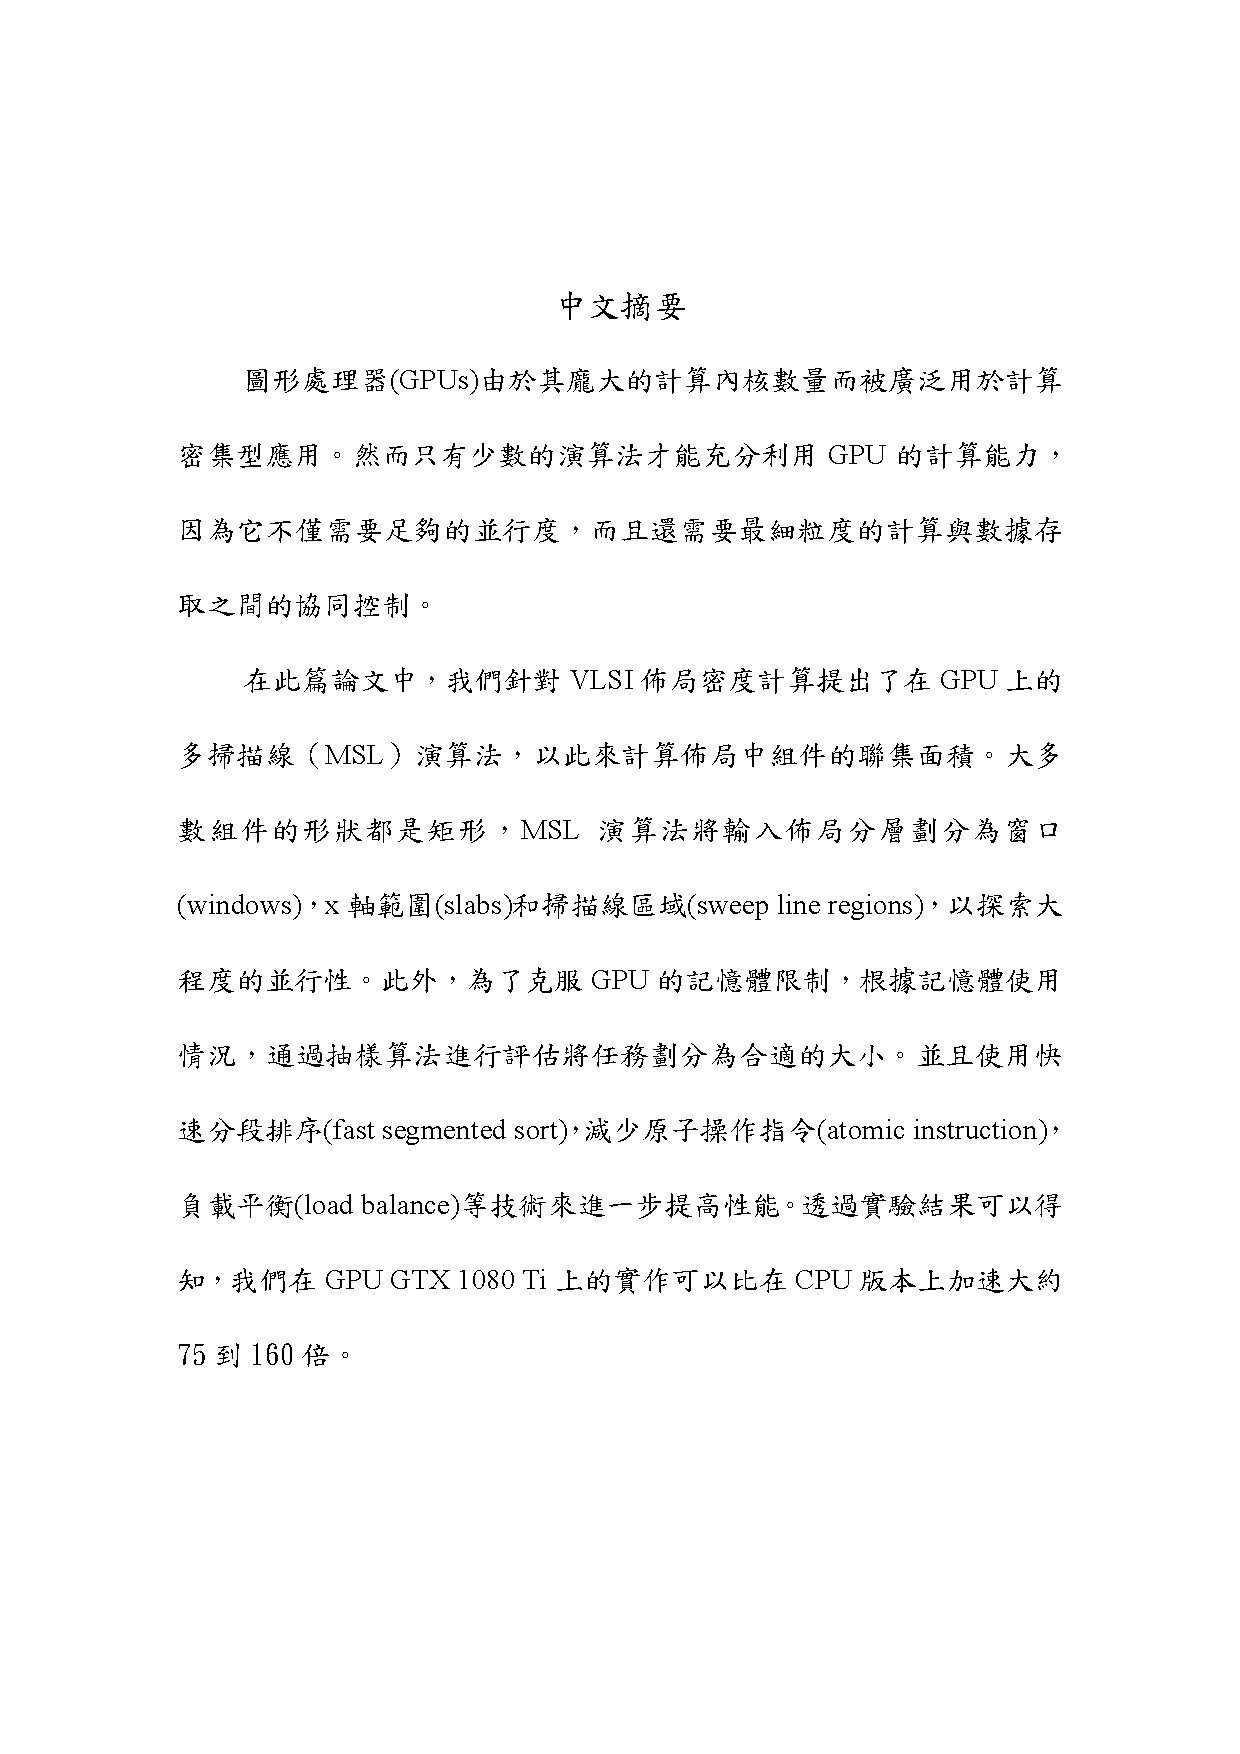
\includepdf[pages={1}]{abstract_ch.pdf}

\addcontentsline{toc}{chapter}{Abstract}
\begin{abstract}
\thispagestyle{plain} 
\setcounter{page}{2}
Graphics Processing Units (GPUs) have been widely used for computational intensive applications owing to its massive number of computing cores.  However, only few algorithms can fully utilize the computational power of GPUs, because it requires not only enough degree of parallelism, but also the synergetic control between computation and data access in the finest granularity.  

%In VLSI (Very-Large-Scale Integration) design, Metal/Pattern density check, which calculates rectangles and vertical trapezoids union area, is required to ensure the mechanical sturdiness of the chip as a whole and to achieve a smooth planar structure for different metal layers so that all metal layers are uniform in structure and performance.  If the metal density is not uniform distributed, some metal layers may be more in height than others and hence the timing, EM, power integrity may be affected.  There are some library, like Boost, providing sequence polygon union function.  However, it is time consuming on CPU, so parallel computing is necessary.  

In this thesis, we proposed the Multi-Sweep-Line (MSL) algorithm on GPU for the VLSI layout density calculation, which computes the union area of components in a layout.  The shapes of most components are rectilinear rectangles. The MSL algorithm divides the input layout hierarchically into windows, slabs, and sweep line regions to explore the large degree of parallelism.  In addition, to overcome the memory limitation of GPU, tasks are partitioned into batches based on memory usage, estimated by sampling algorithms.  Optimization techniques, fast segmented sort, reducing atomic instruction, load balance, are also applied to further improve the performance.   The experimental results show that our MLS implementation can achieve 75 to nearly 160 times speedup over the CPU version on GTX 1080 ti.
\end{abstract}

% IEEEtran.cls defaults to using nonbold math in the Abstract.
% This preserves the distinction between vectors and scalars. However,
% if the conference you are submitting to favors bold math in the abstract,
% then you can use LaTeX's standard command \boldmath at the very start
% of the abstract to achieve this. Many IEEE journals/conferences frown on
% math in the abstract anyway.

% no keywords



%\addcontentsline{toc}{chapter}{Acknowledgements}
%\renewcommand{\abstractname}{Acknowledgements}
\begin{abstract}
\thispagestyle{plain}
\setcounter{page}{3}
There are many people giving assistance on my thesis work. I am very grateful to each of them.
Most of all, I would like to show my deepest gratitude to my advisor, Prof. Che-Rung Lee.
Prof. Lee teaches me how to define problems, map out schedule of implementaion and validation, analyse the result of experiments, optimize the performance and do great presentation.
While discussing problems with Prof. Lee, I learned to use mathematical method to solve problems and proofed the results. In addition, Prof. Lee always helps me find the right direction to overcome difficulties. Therefore, I got more progress in study and also be more delighted on doing research.
Except researching, Prof. Lee provided me the chance to train the junior students to attend Student Cluster Competition. I learned a lot and been inspired while I was teaching and discussing with them.

I would like to express thanks to Dr. I-Hsin Chung, a cooperative partner in IBM, he gave me advises on project and help me learn professional knowledge about my research. Except working, Dr. Chung also teached me the importance of relationship and provided me a chance to get a job in IBM.
And My lab mates also support me on my way of research during the two years. They gave me favors anytime I needed helps. I really appreciate scope lab.

My family always encourage me to achieve my best. I am very grateful to my parents and my brother.
Thanks to all the people around me.

\end{abstract} 

\setcounter{page}{3}
\addcontentsline{toc}{chapter}{Contents}
\tableofcontents
\clearpage
\addcontentsline{toc}{chapter}{List of Figures}
\listoffigures
\clearpage
\addcontentsline{toc}{chapter}{List of Tables}
\listoftables
\clearpage
\addcontentsline{toc}{chapter}{List of Algorithms}
\listofalgorithms
\clearpage


\pagenumbering{arabic}
\setcounter{page}{1}
\chapter{Introduction}
\label{chap:intro}
The deluge of Internet-of-Thing(IoT) create enormous opportunity for machine to recognize the physical
world, the ubiquitous device generate huge size of data at the edge, with the help of deep learning
technique, edge device could extract insight and identify  the surrounding environment. In order to
process these high volume information in real time, processing need to happen near the location
where the data is generated accordingly. However, most of machine learning algorithm and computation device require
significant amount of processing power which may not always be available at the edge.

Autonomous vehicles as one kind of AIoT application have evolved rapidly in the last few
years, which can operate without human control and does
not require any human intervention. As a typical IoT application, self-driving car equipped with
numerous sensor together with GPS and camera. Therefore mutltitple hetergeneous information need to
interpret all together at real time. With leverage on the start-of-art deep learning method 


In this theis, we transport qCUDA, a QEMU + KVM based GPGPU virtualization solution into TX2
development board. qCUDA use API remoting method to submit Nvidia CUDA API from a virtual machine
and bypass it back to host machine to execute the API.The architecture of qCUDA consists of
three parts: library, driver, and virtio virtual device. qCUDA library provide the Nvidia CUDA
interface and analyze the parameter then pass them to qCUDA driver.


%Chapter 4 explains the performance optimization methods developed for the process.
\chapter{Background}
\label{chap:background}
%This is Chapter~ \ref{chap:background} and cite test \cite{Knight:1986:AMF:319838.319854, Sohi:1995:MP:225830.224451, Hammond:1998:DSS:291069.291020}. 


\section{The NVIDIA Jetson TX2}
The NVIDIA Jetson TX2 is a GPU platform targeted at power constrained mobile application. it is designed as an System
on Chip(SoC) which incorporates a quard-core 2.0-GHz 64-bit ARM-v8 A57 processor, a dual-core 2.0-GHz superscalar ARMv8 Denver processor and an integrated Pascal GPU. There are 2MB L2 caches, one shared by the four A57 cores and on shared by the two Denver cores. The GPU has two streaming multiprocessors (SM), each provides 128 1.3-GHz cores that share a 512-KB L2 cache. The six CPU cores and integrated GPU share 8 GB of 1.866-GHz DRAM memory.
 Fig. \ref{fig:fig_2_1} shows the example.
\begin{figure}[!h]
    \centering
    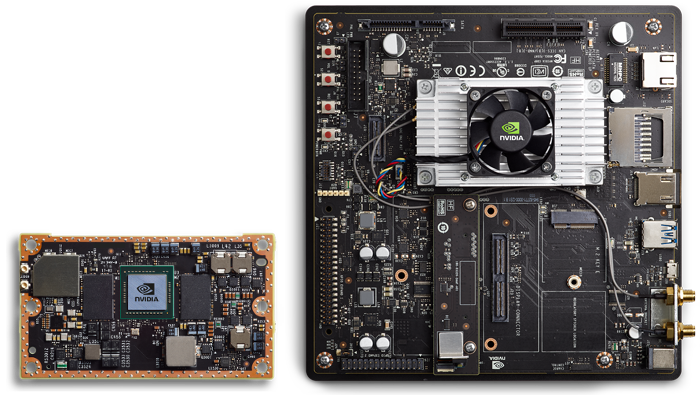
\includegraphics[scale=0.4]{image/jetson_tx2.png}
    \caption{The NVIDIA Jetson TX2 development board}
    \label{fig:fig_2_1}
\end{figure}

\section{Virtualization}
Virtualization refers  to the act of creating a virtual (rather than physical) version of something, includeing  virtual computer hardware platforms, storage devices, and computer network resources. it is a technique that use software to simulate the existence of hardware.
Traditional computing does not allow software to readily share hardware resources. Virtualization
overcomes that limitation by allowing users to run more than one software stack within each virtual system on single physical machine.

This can get greater efficiency of hardware. A virtual computer systems is known as
“virtual machine” (VM): an isolated software machine with an operating system and application
inside. Putting multiple virtual machines on a single computer enables several operating systems and
applications to run on one physical machine. A thin layer of software called a hypervisor which
manages the virtual machines at a physical machine and dynamically allocates computing resources like common processo, memory, I/O and storage to
each virtual machine as needed. 

Early virtualization efforts relied on software emulation to replace hardware functionality. But
software emulation is a slow and inefficient process.

There are three types of virtualization. First is full virtualization, second is para virtualization and third is hardware-assisted virtualization.

\begin{itemize}
    \item full virtualization: The operation system inside the virtual machine  is not aware that it is in a virtualized environment and requires no modification. 
        It use software to emulate all device operation and device driver can be directly installed in the virtual machine. However there are performance overhead and result in performance degradation.
    \item para virtualization : The operation system inside the virtual machine is aware that it is in a virtualized environment and 
        some of components are replaced with optimized one to gain better performance.
    \item hardware-assisted virtualization: An approach  that enables efficient full virtualization using help from hardware capabilities, primarily from the host processors. 
        while the guest must using the same instruction set as the host machine. Hardware-assisted virtualization was added to x86 processors (Intel VT-x or AMD-V) in 2005 and 2006 (respectively).
        Hardware-assisted virtualization reduces the maintenance overhead of paravirtualization as it reduces (ideally, eliminates) the changes needed in the guest operating system. It is also considerably easier to obtain better performance.
\end{itemize}

\section{GPU and NVIDIA CUDA}

Graphics Processing Unit (GPU) is a specialized electronic circuit designed to rapidly manipulate and alter memory to accelerate the creation of images in a frame buffer intended for output to a display device, e.g. personal computers, workstations, game consoles, embedded systems, and some mobile phones. In a personal computer, a GPU can be present on a video card, or it can be embedded on the motherboard, or in certain CPUs, on the CPU die. The term GPU was popularized by Nvidia in 1999. It was presented as a ``single-chip processor with integrated transform, lighting, triangle setup/clipping, and rendering engine''.

The difference between CPU and GPU is their operation method. The CPU consists few cores that used to optimize the sequential sequence processing, like branch condition. The GPU contains thousands of smaller cores to execute the processing of multiple tasks simultaneous. GPUs can be more efficient than general purpose CPUs for algorithms where the processing of large blocks of data is done in parallel because their high parallel structures.

Modern GPUs are very efficient at manipulating computer graphics and image processing, they also play a huge role in many existing applications for physic simulations, media, and machine learning. GPU has accelerated applications in platforms ranging from artificial intelligence to cars, drones, and robots.

Nvidia's Compute Unified Device Architecture (CUDA) platform, first introduced in 2007, was the earliest widely adopted programming model for GPU computing. It allows software developers and software engineers to use a CUDA-enabled graphics processing unit (GPU) for general purpose processing, an approach termed GPGPU (General Purpose computing on Graphics Processing Units). The CUDA platform is a software layer that gives direct access to the GPU's virtual instruction set and parallel computational elements, for the execution of compute kernels. Software developers, scientists and researchers have applied CUDA to variety fields, such as image and video processing, computational biology and chemistry, fluid dynamics simulation, CT image reconstruction, seismic analysis, traceability, etc.. The CUDA platform is designed to work with programming languages such as C, C++, and Fortran. Also, CUDA supports programming frameworks such as OpenACC and OpenCL.

In the CUDA program, there are two different computing environments, which are called host and device. Host is the computing environment of original central processing unit, and device is the GPU, which has independent memory and computing cores. Fig. \ref{fig:fig_2_4} shows the simple flow chart in CUDA programming. First, the data for calculation is transformed form host to device; second, host call GPU functions; and then device deals with the data and finally copy the result back to host. CUDA express Single Instruction Multiple Data (SIMD) parallelism, there are thousands of threads in the kernel to execute the same code. Each thread will belong to a thread block and share the shared memory. The total number of threads in the same blocks has an upper limit (not more than 1024 threads in general). All the blocks will belong to a grid and can access the whole the global memory. Each thread and block has a different assigned number, called thread ID and block ID, according to the different order. And each thread can access different data for processing by way of their thread ID.
\begin{figure}[h]
    \centering
    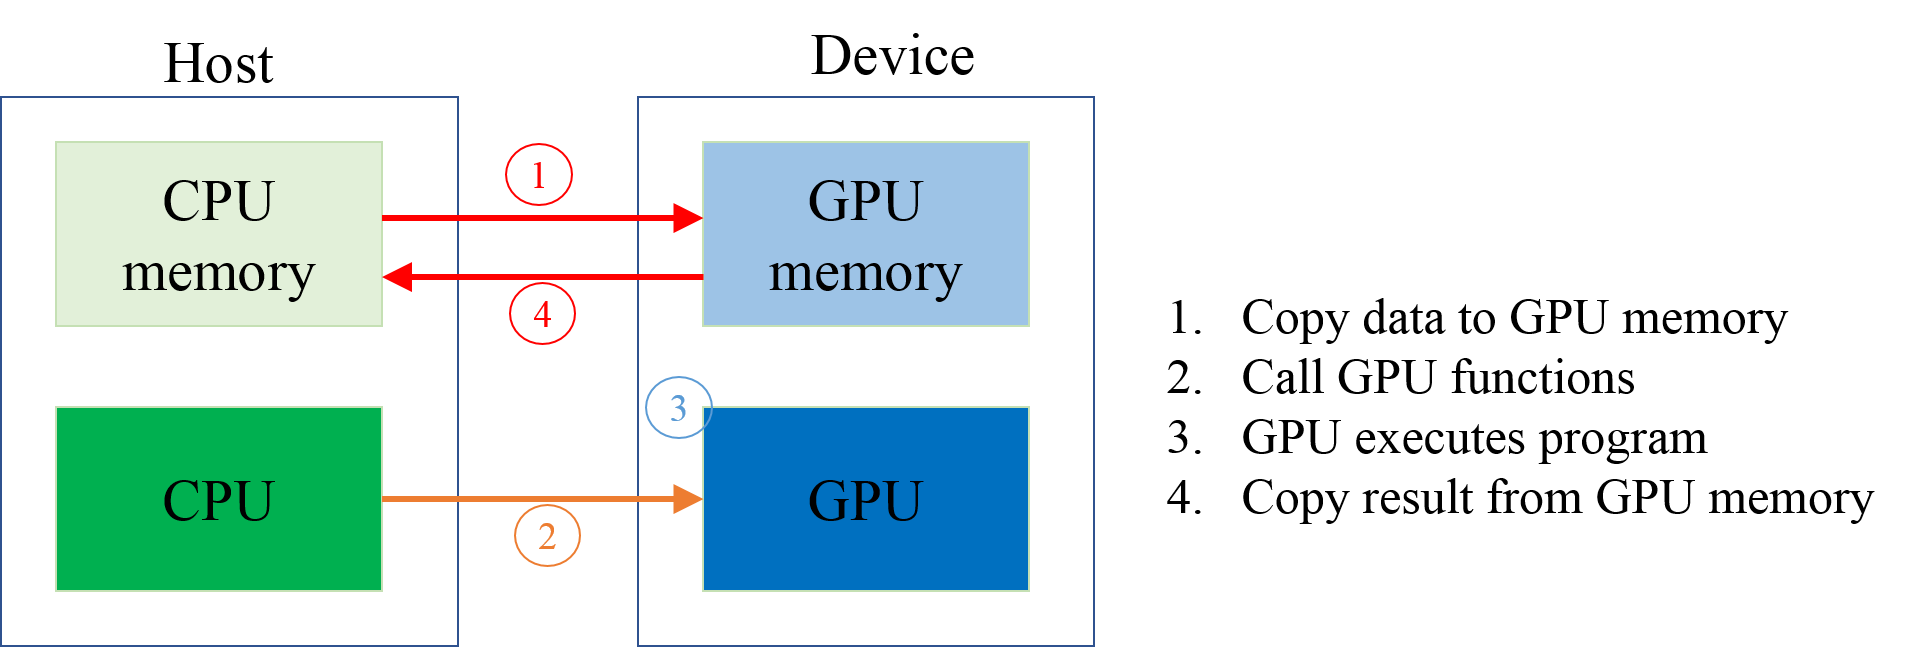
\includegraphics[scale=0.5]{image/fig_2_4}
    \caption{The simple flow chart of CUDA programming}
    \label{fig:fig_2_4}
\end{figure}

When the kernel is launched from the host, system creates many threads on GPU that executes simultaneously. The threads share the same program counter in the same warp. A warp consists 32 threads; warps are grouped into a block; blocks are grouped into a grid.

The \_\_shfl intrinsics permit exchanging of a variable between threads within a warp without use of shared memory. The exchange occurs simultaneously for all active threads within the warp (and named in mask), moving 4 or 8 bytes of data per thread depending on the type. Threads may only read data from another thread which is actively participating in the \_\_shfl command. If the target thread is inactive, the retrieved value is undefined.

Another keyword is atomic. An atomic function performs a read-modify-write atomic operation on one 32-bit or 64-bit word residing in global or shared memory. The operation is atomic in the sense that it is guaranteed to be performed without interference from other threads. In other words, no other thread can access this address until the operation is complete. Atomic functions do not act as memory fences and do not imply synchronization or ordering constraints for memory operations.

The more detail can be found on cuda programming guide \cite{cuda_programming_guide}.

\section{Related research}
Polygon operation is an important technique in Geographic Information Systems (GISs) and Very-Large-Scale-Integration (VLSI) design. In general polygon union, the common method is overlay polygons and calculate the generated polygons. Oosterom \cite{Peter:1994} presented a vector map-overlay algorithm used R-tree. Boost \cite{Simonson2009GeometryTL} \cite{Schling:2011:BCL:2049814} provides open source library to do the basic polygon operations. However, it is usually time consuming. Parallel algorithms used in VLSI design bring significant challenges for their efficient and effective implementation. Prasad et. al. \cite{Prasad:2015:GPR:2863697.2864578} presented a space-efficient data structure design and a non-trivial bottom-up construction algorithm for R-tree on GPUs. McKenney et. al. \cite{McKenney:2011:GOC:2093973.2094051} used a brute force approach to compute the line segment intersection. Wang et. al. presented a hybrid CPU-GPU approach which can be used to find the intersection and union of polygons represented in pixel format.

The plane sweep algorithm has also received many investigations since it forms the foundation of many common spatial operations, e.g. rectangle intersection in polygon operations and line segment intersection.
In 2009, McKenney et. al. \cite{McKenney2009APP} presented a parallel version of the plane sweep algorithm, which targeted towards the small number of processing cores available on commonly available multi-core systems. The overall design of their algorithm has three steps: (1) an initial scan equally slices the input data into p strips; (2) plane sweep algorithms run over each strip in parallel; (3) the result of the plane sweeps are merged into a result. Qiu et. al. \cite{Qiu2013APS} used Message-Passing-Interface (MPI) as the programming model, which is commonly used in the distributed memory architecture, to compute the line segments intersection by efficient and robust parallel plane sweep algorithm. Khlopotine et. al. \cite{Khlopotine2013AVO} presented a variant of a plane sweep algorithm to calculate the rectangle intersection and used OpenMP to enable parallel execution of the algorithm. Lo et. al. \cite{Lo2013OptimizingPB} provided a parallel algorithm to perform Pairwise Box Intersection checking on GPUs (PBIG). The PBIG algorithm consists of three phases: planning, mapping and checking. The planning phase partitions the space into small cells, the sizes of which are determined to optimize performance. The mapping phase maps the rectangles into the cells. The checking phase examines the rectangles intersections in the same cell. Several performance optimization techniques, including load-balancing, output data compression/encoding, and pipelined execution, are presented in the paper.

\chapter{Multi-Sweep-Line Algorithm}
\label{chap:methodology}
In this chapter, we formally present the problem and describe our parallel implementations. 

%Version 1 uses line sweep algorithm straightforward. Version 2 makes modifications based on version 1. In our implementation, we calculate the union area of rectangles on GPU and the triangles on CPU.

\section{Problem definition}
The input is a layout of VLSI design, which is a two dimensional rectangle space called a cell.  A cell is further subdivided into equal sized windows, whose width and height are equal to window size.  The window stride means the distance between two adjacent windows.  Inside the layout, components are decomposed as rectangles and triangles. The problem is to calculate the layout density of each window, which is the ratio of the area covered by rectangles and triangles. We only consider the union of rectangles here, and will discuss the process of union of triangles later.  Figure \ref{fig:fig_3_1} gives an example, in which the size and the stride of windows are the same.

\begin{figure}[!h]
    \centering
    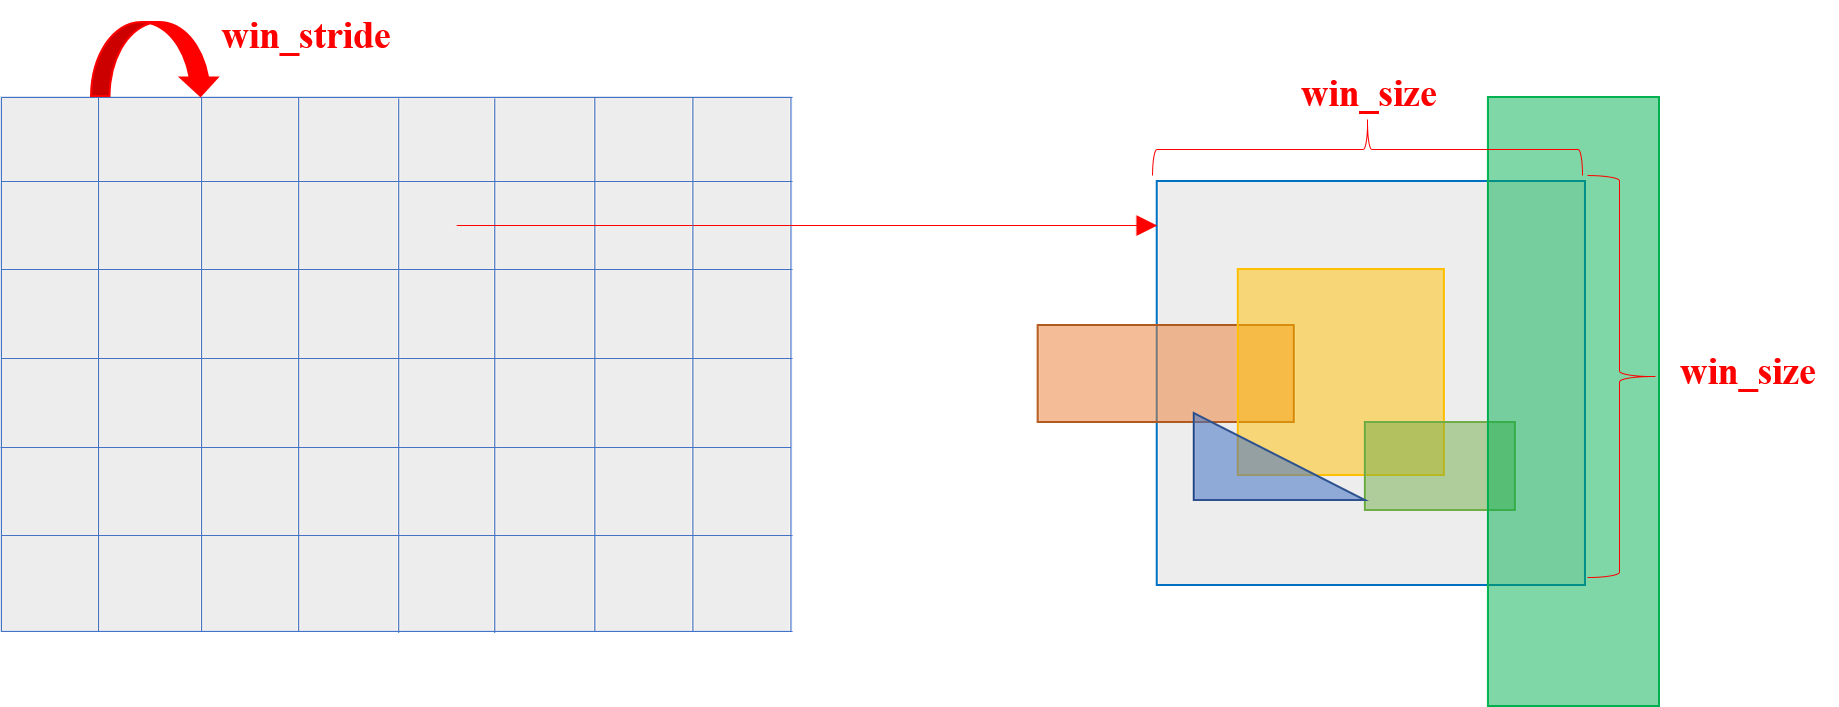
\includegraphics[scale=0.4]{image/fig_3_1}
    \caption{Cell, windows (window's stride is equal to size in this diagram), rectangles, and triangles}
    \label{fig:fig_3_1}
\end{figure}

\section{High Level Description}
% how to parallelize v1 v2 v3
In this section, we describe our three parallel implementations: baseline, multi-slab, and multi-sweep-line in high level.

\subsection{Baseline Algorithm}
Our baseline version is embarrassing parallelization. A layout can be partitioned into windows, so we can compute the union of rectangles for each window in parallel. In baseline version, we use sweep line algorithm and directly port it to GPU. The pseudo code is shown in Algorithm \ref{alg:a2}. To reduce the memory usage, we do not save y value. 

\begin{algorithm}[H]
\label{alg:a2}
\caption{Baseline: sweep line algorithm directly porter}
\DontPrintSemicolon
\renewcommand\baselinestretch{0.7}\selectfont
 \KwData{$R$: a list of rectangles for each window}
 \KwResult{Each window's area of rectangle union}
 \SetKwProg{Fn}{Function}{}{}
 \SetKwFunction{FMain}{main}
 \SetKwProg{Pn}{Function}{:}{\KwRet}
 \Pn{\FMain}{
     sort the x value of rectangles for each window\;
     sort each window's rectangles based on y\;
     \bf{parallel} \ForEach{$W_j \in W$}{
         $area = 0$\;
         \bf{parallel} \ForEach{$slab (x[i-1], x[i])$}{
             compute\_area($x[i-1], x[i]$)\;
         }
     }
 }
 \;
 \Pn{compute\_area($x1, x2$)}{
    Let $R[k]$ be the first rectangle in $[x1, x2]$\;
    begin = R[k].ymin\;
    end = R[k].ymax\;
    \ForEach{$r \in R$}{
        \If{$r$ is in $[x1, x2]$}{
            \uIf{$r.ymin <= end$}{
                $end = max(r.ymax, end)$\;
            }
            \Else{
                $area += (end - begin) * (x2 - x1)$\;
                $begin = r.ymin$\;
                $end = r.ymax$\;
            }
        }
    }
 }
\end{algorithm}

\subsection{Multi-Slab Algorithm}
The function of computing\_area in baseline version (naive parallelization) is the performance bottleneck because each thread checks all rectangles in a window, whether a rectangle is in the slab or not. It is ineffective for GPU architecture. For this reason, we modified the implement by changing threads' task. Each thread now handles one slab and only checks the rectangles in this slab. The pseudo code of compute\_area function is shown in Algorithm \ref{alg:a3}.

\begin{algorithm}[H]
\label{alg:a3}
\caption{Multi-slab: modify bottleneck in baseline and task partition}
\DontPrintSemicolon
\renewcommand\baselinestretch{0.7}\selectfont
 \KwData{$R$: a list of rectangles for each window}
 \KwResult{Each window's area of rectangle union}
 \SetKwProg{Fn}{Function}{}{}
 \SetKwFunction{FMain}{main}
 \SetKwProg{Pn}{Function}{:}{\KwRet}
 \Pn{\FMain}{
     sort the x value of rectangles for each window\;
     sort each window's rectangles based on y\;
     create active list for each slab each window\;
     \bf{parallel} \ForEach{$W_j \in W$}{
         $area = 0$\;
         \bf{parallel} \ForEach{$slab (x[i-1], x[i])$}{
             compute\_area($x[i-1], x[i]$)\;
         }
     }
 }
 \;
 \Pn{compute\_area($x1, x2$)}{
    Let $r1$ be the first rectangle in $[x1, x2]$\;
    begin = r1.ymin\;
    end = r1.ymax\;
    \ForEach{$r \in R$}{
        \uIf{$r.ymin <= end$}{
            $end = max(r.ymax, end)$\;
        }
        \Else{
            $area += (end - begin) * (x2 - x1)$\;
            $begin = r.ymin$\;
            $end = r.ymax$\;
        }
    }
 }
\end{algorithm}

\subsection{Multi-Sweep-Line Algorithm}
In the function of compute\_area in multi-slab version, each thread handles a slab and scan all rectangles within this slab. It is faster than the compute\_area function in baseline version. However, it suffers from the discontinuous memory access. So we present multi-sweep-line algorithm to speed up the computing time in compute\_area function. The pseudo code of compute\_area function is shown in Algorithm \ref{alg:a4}.

\begin{algorithm}[H]
\label{alg:a4}
\caption{The compute\_area function in multi-sweep-line which is optimized from multi-slab version}
\DontPrintSemicolon
\renewcommand\baselinestretch{0.7}\selectfont
\SetKwProg{Pn}{Function}{:}{\KwRet}
 \Pn{compute\_area($x1, x2$)}{
    //multi sweep line\;
    warp (32 thread) task:\;
    each warp handles a slab\;
    \While{choose 32 rectangles}{
        each thread handles a rectangle\;
        check rectangles before this thread\;
        add result to area\;
    }
 }
\end{algorithm}

%%%%%%%%%%%%%%%%%%%%%%%%%%%%%%%%%%%%%%%%%%%%%%%%%%5
\section{GPU Implementation}
In this section, we describe our three parallel implementations: baseline, multi-slab, and multi-sweep-line more detailed.

\subsection{Baseline Algorithm}
The layout density calculation can be parallelized embarrassingly by computing the density of each window in parallel, and then aggregating all the results.  We designed an effective GPU implementation for this method so that we can use it as the baseline for comparison.  The implementation uses four global arrays:
\begin{itemize}
    \item Counter Array ($C$): whose size equals to the number of windows.  Element $C[i]$ records the number of rectangles in window $i+1$.
    \item Offset Array ($O$): whose size also equals to the number of windows.  Elements in $O$ represent the indices of Rectangle Array ($R$).  
    \item Rectangle Array ($R$): whose size equals to the total number of rectangles in all windows, $\sum_{i=1}^n C[i]$.  The IDs of rectangles in window $i$ are stored in $R$ from index $O[i-1]$ to index $O[i]-1$, or to the last element of $R$.
    \item X\_range Array ($X$): whose size is double of that of $R$. It stores the x coordinates of two end points of rectangles in each window.
\end{itemize}
Fig. \ref{fig:fig_3_3} shows an example of those data structures.  
\begin{figure}[h]
    \centering
    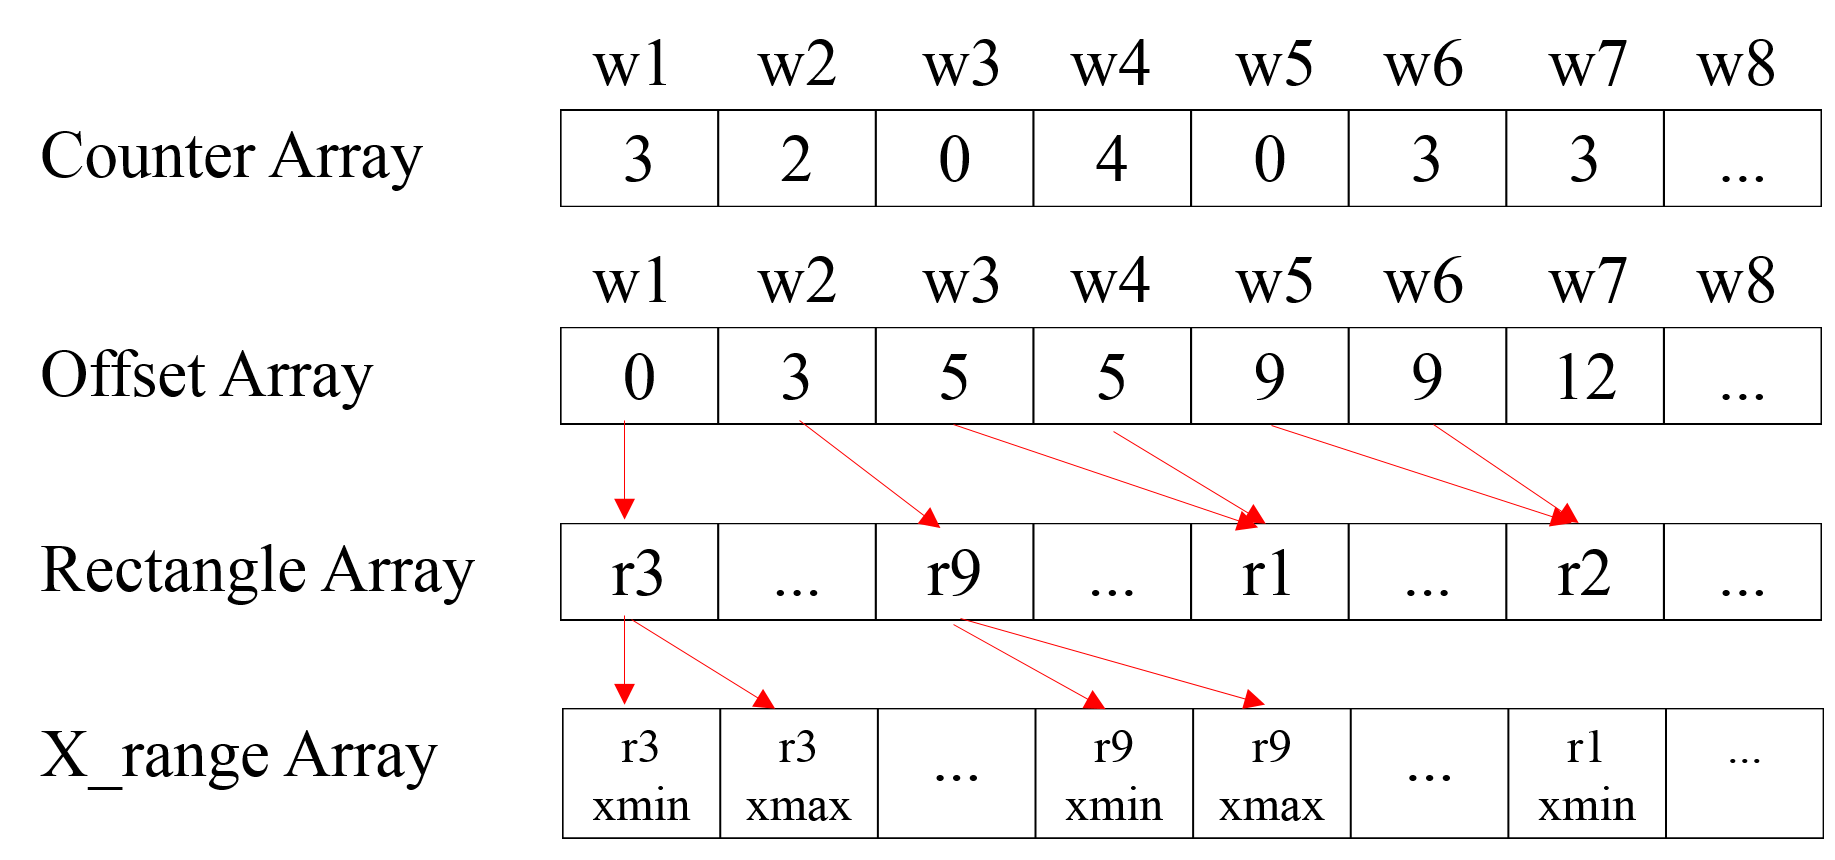
\includegraphics[scale=0.4]{image/fig_3_3}
    \caption{Example of the counter, offset, rectangle, and x\_range array. Rectangles are concatenated in the rectangle array according to the cell order}
    \label{fig:fig_3_3}
\end{figure}


The algorithm consists of three phases: counting phase, mapping phase, and computing phase.  The first two phases enumerate the rectangles appeared in each window and store their information using those four arrays.  The rectangles are sorted first based on their y coordinates, so the algorithm can process the rectangles sequentially later.  The last step calculates the area union of rectangles.

The counting phase counts the number of rectangles in each window.  Each thread handles a rectangle and computes which windows it occupies.  If a rectangle appears in window $i$, the thread increases the $i$th element of the \textit{counter array} $C$ using atomic instructions.

The target of mapping phase is to fill the \textit{rectangle array} with rectangles' ID. First, it uses the \textit{counter array} and performs parallel prefix sum algorithm (scan) \cite{ref} to generate the \textit{offset array}. Second, it fills the \textit{rectangle array} with rectangles' ID. The position of a rectangle in the \textit{rectangle array} is the \textit{offset array} of the window.  Each thread handles a rectangle and performs one atomic add instruction to obtain the correct order in the \textit{rectangle array}.  When filling the rectangle to the \textit{rectangle array}, it also fills the \textit{x\_range array}.  Finally, the algorithm sorts every segment of the \textit{rectangle array} and the \textit{x\_range array} to ensure the order of rectangles and slabs. 

The computing phase uses sweep line algorithm to calculate the density of rectangles in each window. Each block processes four windows.  Each thread picks one slab to compute the union area and repeats the action until all slab are computed. Every thread reads the information of all the rectangles in the window. If the rectangle is not appeared on the range (slab), the thread will ignore it. When sweeping rectangles in the window, each thread performs one atomic instruction to shared memory to record the area covered by rectangles. Finally, the algorithm writes the answer from the shared memory to the global memory.
\begin{figure}[h]
    \centering
    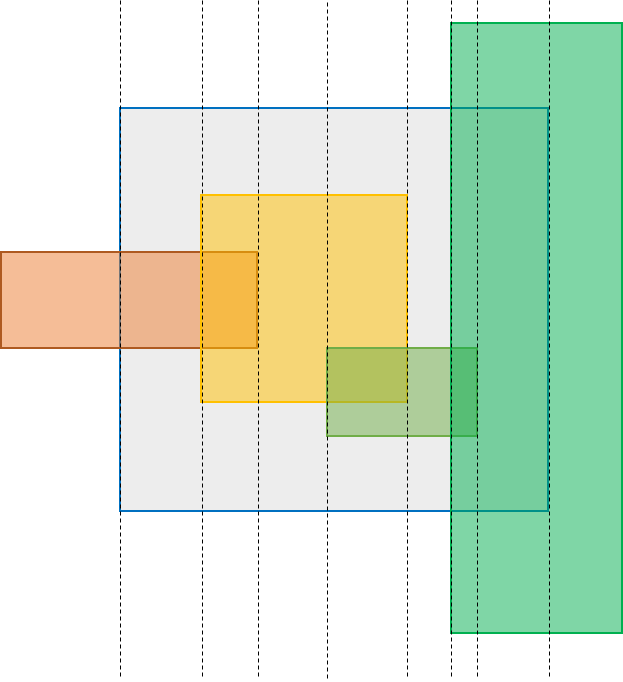
\includegraphics[scale=0.4]{image/fig_3_4}
    \caption{Computing phase: each thread handles a slab (between two dash line)}
    \label{fig:fig_3_4}
\end{figure}


The bottleneck of the baseline algorithm is in the computing phase because each thread needs to check all rectangles in a window, whether they are in the slab or not.  

\subsection{Multi-Slab Algorithm}
The computing phase in baseline version (naive parallelization) is the performance bottleneck because each thread checks all rectangles in a window, whether a rectangle is in the slab or not. It is ineffective for GPU architecture. For this reason, we modified the implement by changing threads' task. Each thread now handles one slab and only checks the rectangles in this slab.

Our target is to generate an array to store the concatenated rectangles lists for all slabs for all windows. For this purpose, three additional arrays are used. First, the \textit{range rectangle array} stores the concatenated rectangles lists for all slabs for all windows. Second, the \textit{range offset array} records the beginning address of each rectangle list in the \textit{range rectangle array}. Third, the \textit{range counter array} keeps the number of rectangles in each slab for all windows. Fig. \ref{fig:fig_3_5}a shows the flow chart of multi-slab version. Multi-slab version consists of five phases, which are described as follows:
\begin{figure}[h]
    \centering
    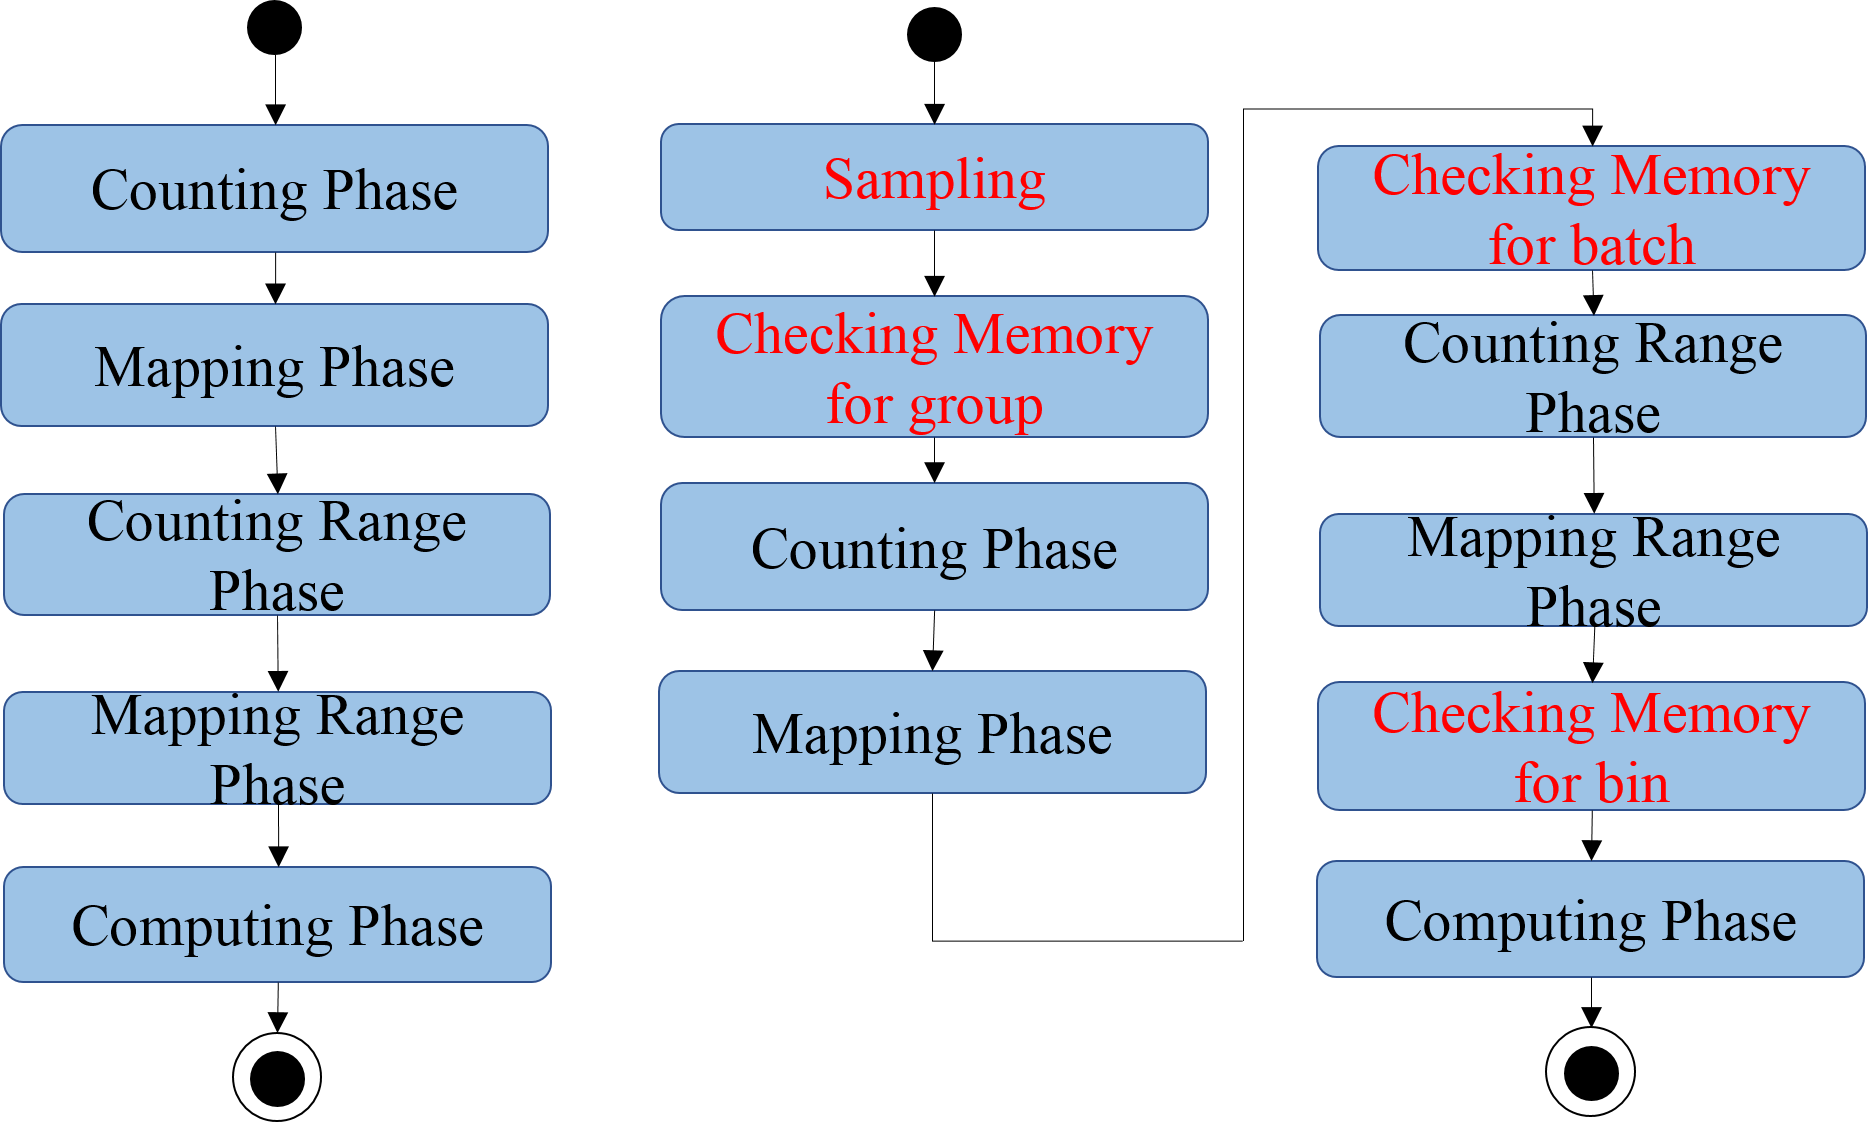
\includegraphics[scale=0.4]{image/fig_3_5}
    \caption{(a) The flow chart of multi-slab and multi-sweep-line without checking memory (b) The flow chart of multi-slab and multi-sweep-line with checking memory}
    \label{fig:fig_3_5}
\end{figure}

\subsubsection{Counting phase}
Same as the counting phase in baseline version.

\subsubsection{Mapping phase}
Same as the mapping phase in baseline version.

\subsubsection{Counting range phase}
The main task of counting range phase is counting the number of rectangles for each slab per window. We unique the \textit{x\_range array} and sort it to compute how many slabs per window before perform the main task. And then counting the number of rectangles. Like the counting phase in baseline version, each thread handles one rectangle in this window and computes the ranges it occupies. For an occupied range of index $i$, the thread increases the $i$th element in the \textit{range counter array} using atomic instruction to avoid race condition.

\subsubsection{Mapping range phase}
Unlike the counting range phase, each thread handles one slab instead of one rectangle. It can keep the order of rectangles in this slab. We need to spend much time to sort the \textit{range rectangle array} if each thread handles one rectangle using atomic instruction.

\subsubsection{Computing phase}
Same as the computing phase in baseline, but every thread only checks all rectangles within a slab.

\subsection{Multi-Sweep-Line Algorithm}
In computing phase in multi-slab version, each thread handles a slab and scan all rectangles within this slab. It is faster than computing phase in baseline version. However, it suffers from the discontinuous memory access: (1) we need to read rectangle's information and rectangles' information only sorted according to their y coordinate; (2) each thread in same warp (32 threads) access rectangle's index in \textit{range rectangle array} is not continuous because each thread handles different slabs. First condition cannot be fixed unless we save rectangles' value to range rectangle array instead of rectangles' index. This way will use amount of memory and memory is rare resource. In this optimization technique, we solve the problem in the second condition.

We modify the implementation in computing phase. Original sweep line algorithm scan rectangles one by one. We now scan 32 (size of warp in CUDA) rectangles in one time. We let each warp handle a slab and each thread in the same warp handles a rectangle, compare the value of the status variable (the value of statue is window's smaller y coordinate in the beginning), and check the rectangles (these rectangles' ymax) which are handled by the threads that their thread ID is smaller than its. After checking rectangles, each thread computes the area and adds the result to local variable. The final thread in this warp has maximum y coordinate value and update the status. After that, warp handles next 32 rectangles in this slab. Fig. \ref{fig:fig_4_2} shows the example.
\begin{figure}[h]
    \centering
    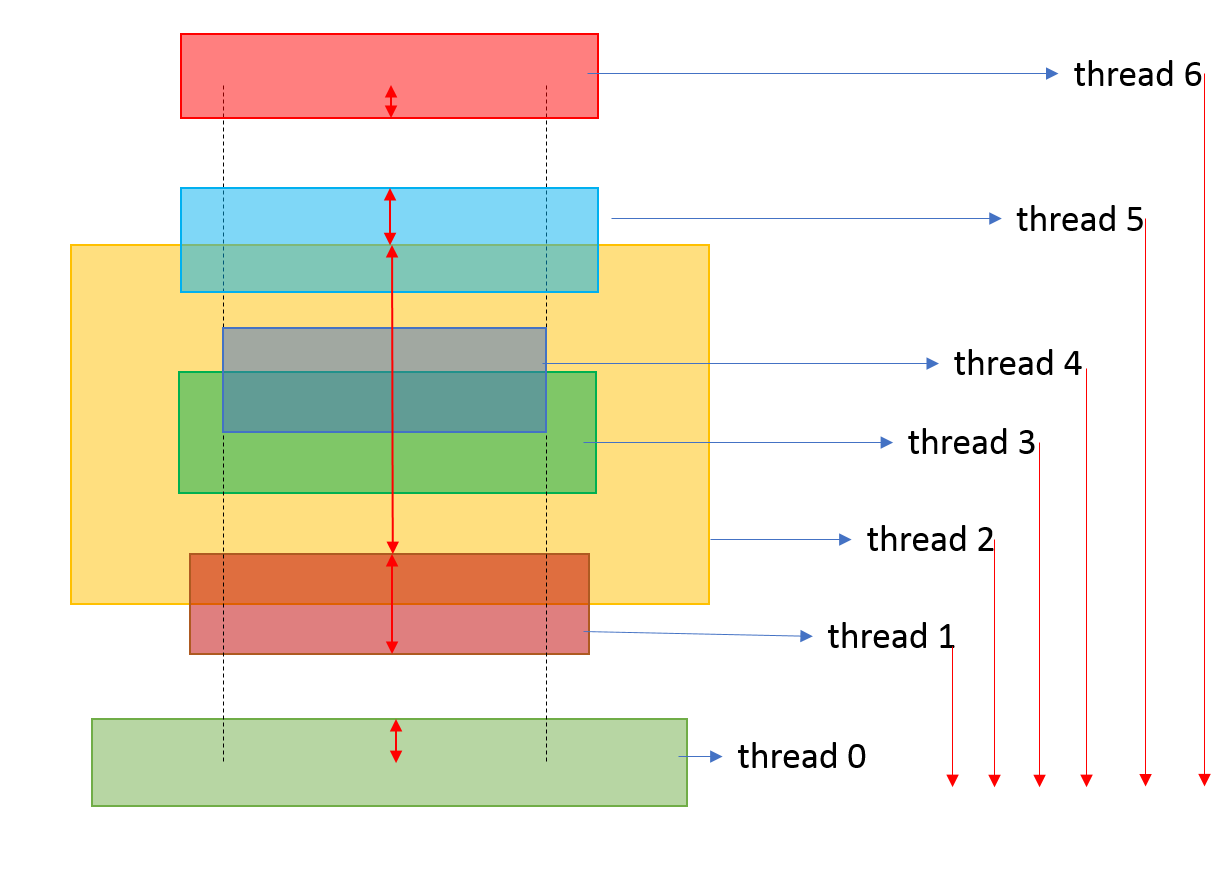
\includegraphics[scale=0.4]{image/fig_4_2.png}
    \caption{Example of computing phase using multi-sweep-line, each thread in same warp handles a rectangle in same slab (each red arrow are calculated by certain thread)}
    \label{fig:fig_4_2}
\end{figure}

% adaptive memory partition
\subsection{Checking and adaptive task partition}
The computing phase time in multi-slab and multi-sweep-line version is faster than baseline version, but it uses a lot of GPU memory to save additional arrays (i.e. the \textit{range counter array}, the \textit{range offset array}, and \textit{range rectangle array}). For example, certain test cases will generate a \textit{range rectangle array} about 60 GB. There is no such a GPU has enough global memory to store the array in one time. To solve this problem, we designed an adaptive partition method. (see Fig. \ref{fig:fig_3_5}b) The unit of our partition method is window, Fig. \ref{fig:fig_3_8} shows the schematic diagram. The pseudo code is shown in Algorithm \ref{alg:a5}.

\begin{figure}[h]
    \centering
    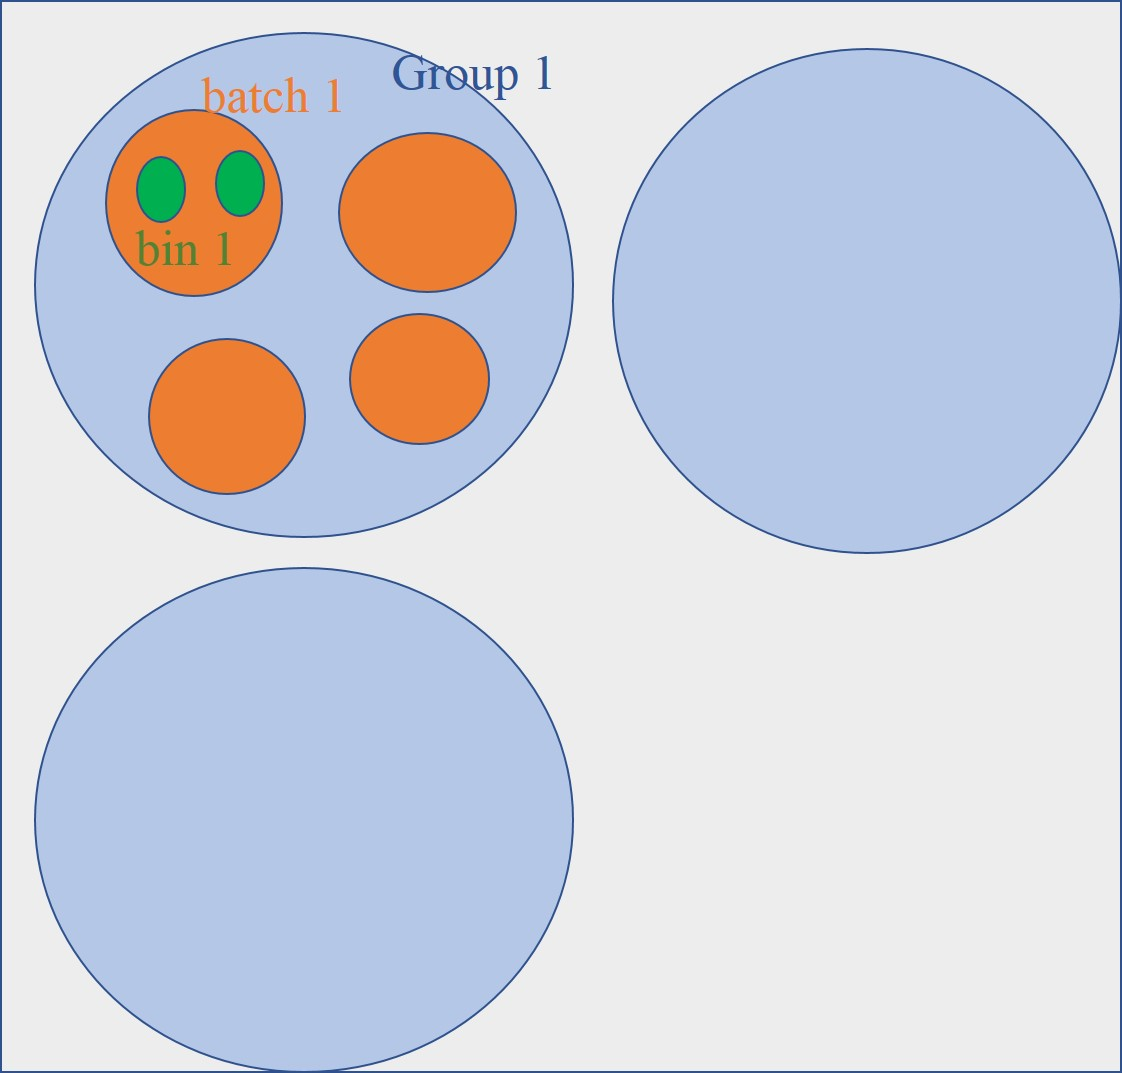
\includegraphics[scale=0.4]{image/fig_3_8.jpg}
    \caption{The schematic diagram of partition method (group, batch, and bin), which the unit is window}
    \label{fig:fig_3_8}
\end{figure}

\begin{algorithm}[H]
\label{alg:a5}
\caption{Multi-slab and multi-sweep-line with checking memory}
\DontPrintSemicolon
\renewcommand\baselinestretch{0.7}\selectfont
 \KwData{$R$: a list of rectangles for each windows}
 \KwResult{Each window's area of rectangle union}
 \SetKwFunction{FMain}{main}
 \SetKwProg{Pn}{Function}{:}{\KwRet}
 \Pn{\FMain}{
     sampling\;
     \#groups = Checking memory for windows\;
     \ForEach{group of windows}{
         sort the x value of rectangles for each window\;
         sort each window's rectangles based on y\;
         \#batch = Checking memory for slabs\;
         \ForEach{batch of windows}{
             create range\_counter array for each slab\; 
             create range\_offset array for each slab\;
             \#bin = Checking memory rectangles\;
             \ForEach{bin of windows}{
                 create range\_rectangle array for each slab\;
                 \bf{parallel} \ForEach{$W_j \in W$}{
                     $area = 0$\;
                     \bf{parallel} \ForEach{$slab (x[i-1], x[i])$}{
                         compute\_area($x[i-1], x[i]$)\;
                     }
                 }
             }
         }
     }
 }
\end{algorithm}

\subsubsection{Sampling}
\begin{table}[h!]
\centering
\begin{tabular}{|c | l |} 
 \hline
 Symbol & Meaning \\ [0.5ex] 
 \hline
 $\alpha$ & average number of rectangles per window  \\
 $\beta$ & average number of rectangles per slab in the window  \\
 $\gamma$ & average number of windows that a rectangle occupies  \\
 $N$ & number of total rectangles \\
 $M$ & number of total windows  \\ \hline
 $l^i_c$ & length of cell in the $i$th dimension  \\
 $l^i_r$ & length of rectangle in the $i$th dimension  \\ \hline
 $win\_size$ & length of each window  \\
 $win\_stride$ & interval between two adjacent windows  \\
 \hline
\end{tabular}
\caption{List of Symbols}
\label{table:symbol}
\end{table}
The memory usage in whole process we estimate is approximate $(6M + 11\alpha M + (2\alpha - 1) M\beta)$ 32 bits ($(2\alpha - 1)$ means average of maximum number of slabs in each window), where $M$ is the number of windows, $\alpha$ is the average number of rectangle per window, and $\beta$ is the average number of rectangles per slab in the window.

Given the window's size, window's stride, and the size of $l^1_c \times l^2_c$, where $l^i_c$ is the length of cell in the $i$th dimension and symbol stands for the multiplication sign between scalars, $M$ can be calculated as
\begin{equation}
M = \left(\left\lceil{\frac{l^1_c - win\_size}{win\_stride}}\right\rceil + 1\right) \times \left(\left\lceil{\frac{l^2_c - win\_size}{win\_stride}}\right\rceil + 1\right).
\end{equation}
Similarly, given the size of a rectangle r $l^1_r \times l^2_r$, where $l^i_r$ is the length of r in the $i$th dimension and symbol stands for the multiplication sign between scalars, the number of windows occupied by r can be estimated using
\begin{equation}
\left(\left\lceil{\frac{l^1_r - win\_size}{win\_stride}}\right\rceil + 1\right) \times \left(\left\lceil{\frac{l^2_r - win\_size}{win\_stride}}\right\rceil + 1\right) \mbox{, if $l^i_c > win\_size$}.
\end{equation}
Thus, $\gamma$ is defined as 
\begin{equation}
\gamma = \frac{1}{N}\sum_{r \in R} \left(\left(\left\lceil{\frac{l^1_r - win\_size}{win\_stride}}\right\rceil + 1\right) \times \left(\left\lceil{\frac{l^2_r - win\_size}{win\_stride}}\right\rceil + 1\right)\right),
\end{equation}
where $R$ denotes the set of $N$ rectangles in the cell. Then, $\alpha$ can be computed as 
\begin{equation}
\alpha = \frac{N * \gamma}{M}
\end{equation}
To reduce the calculational cost and increase accuracy, we take a simple random sample of size 1024 from $M$ windows to estimate $\alpha$ and offload sampling phase onto the GPU.

Based on the same consideration, we using $\alpha$ to estimate $\beta$ instead of calculating $\beta$ using sample method. We assume average number of slabs is $(2\alpha - 1)$ per window (because each window evenly has $\alpha$ rectangles). The value of $\beta$ is between $\frac{\alpha}{2\alpha-1} \sim \frac{\alpha^2}{2\alpha-1}$, which means best case and worst case(like Fig. \ref{fig:fig_3_6}). And we take the middle of these two number to denote $\beta$.
\begin{figure}[h]
    \centering
    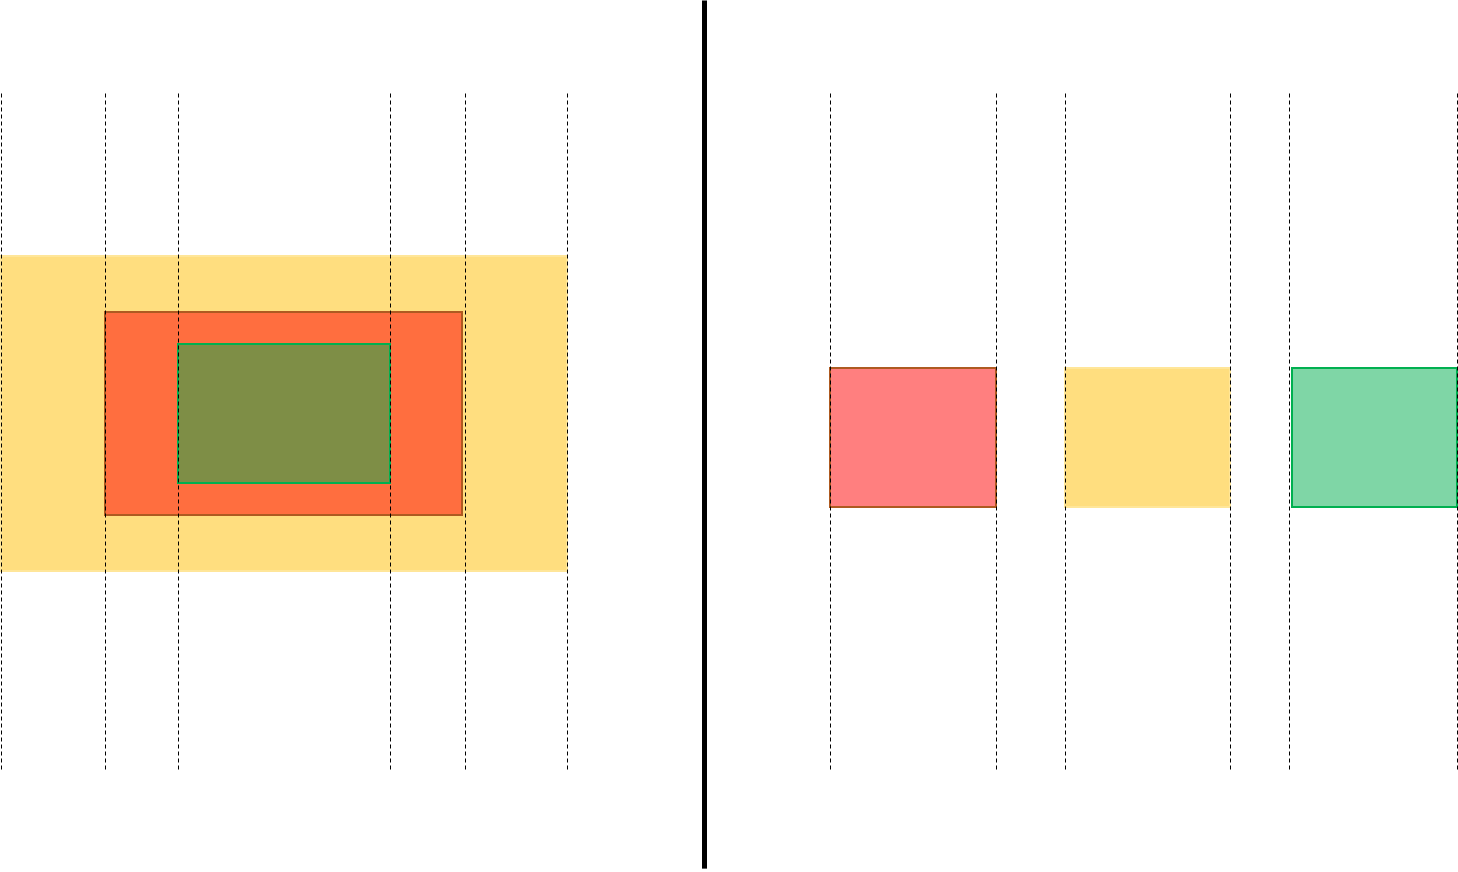
\includegraphics[scale=0.4]{image/fig_3_6}
    \caption{One of the worst case (left) and best case (right) of overlapping}
    \label{fig:fig_3_6}
\end{figure}

\subsubsection{Checking memory for windows (group)}
Using $\alpha$ can estimate total memory usage except \textit{range rectangle array}, \textit{range offset array} and \textit{range counter array} (because these arrays almost larger than GPU memory, and we check these three arrays in checking memory for slabs and rectangles). If memory is not enough, we partition windows equally.

\subsubsection{Checking memory for slabs (batch)}
If memory is not enough for \textit{range counter array} and \textit{range offset array}, this phase will use $\beta$ to determinate how many parts does the workload be divided and adaptive partition task. We use $\beta$ to make a decision because we do not want the process partition task in checking memory 3 phase after divide the work in this phase.

\subsubsection{Checking memory for rectangles (bin)}
If \textit{range rectangle array} is larger than free memory, this phase will adaptive partition task according to \textit{range offset array}.

It should be noted that we do not remove any array, which is complete computed before checking memory for slabs or for rectangles, because all the information can be reuse and we do not want to repeat the calculation.

%%%%%%%%%%%%%%%%%%%%%%%%%%%%%%%%%%%%%%%%%
\section{Performance Optimization}
In this section, we present three optimization techniques to further enhance the GPU performance. The first technique uses fast segmented sort to speed up the sorting time. The second technique reduces the usage of atomic instruction which can break performance. The third technique modifies the implementation of computing phase in multi-sweep-line version to improve the performance.
% segment sort
\subsection{Fast segmented sort}
Hou et. al. \cite{Hou2017FastSS} presented an adaptive segmented sort mechanism for GPUs, whose key techniques contain: (1) a differentiated method for different segment lengths to eliminate load imbalance, thread divergence, and irregular memory access; and (2) an algorithm that extends sorting networks to support N-to-M data-thread binding and thread communication at GPU register level. Fig. \ref{fig:fig_4_1} shows the overview of their design. We modify their source code and integrate our algorithm with it to speed up the sorting time.
\begin{figure}[h]
    \centering
    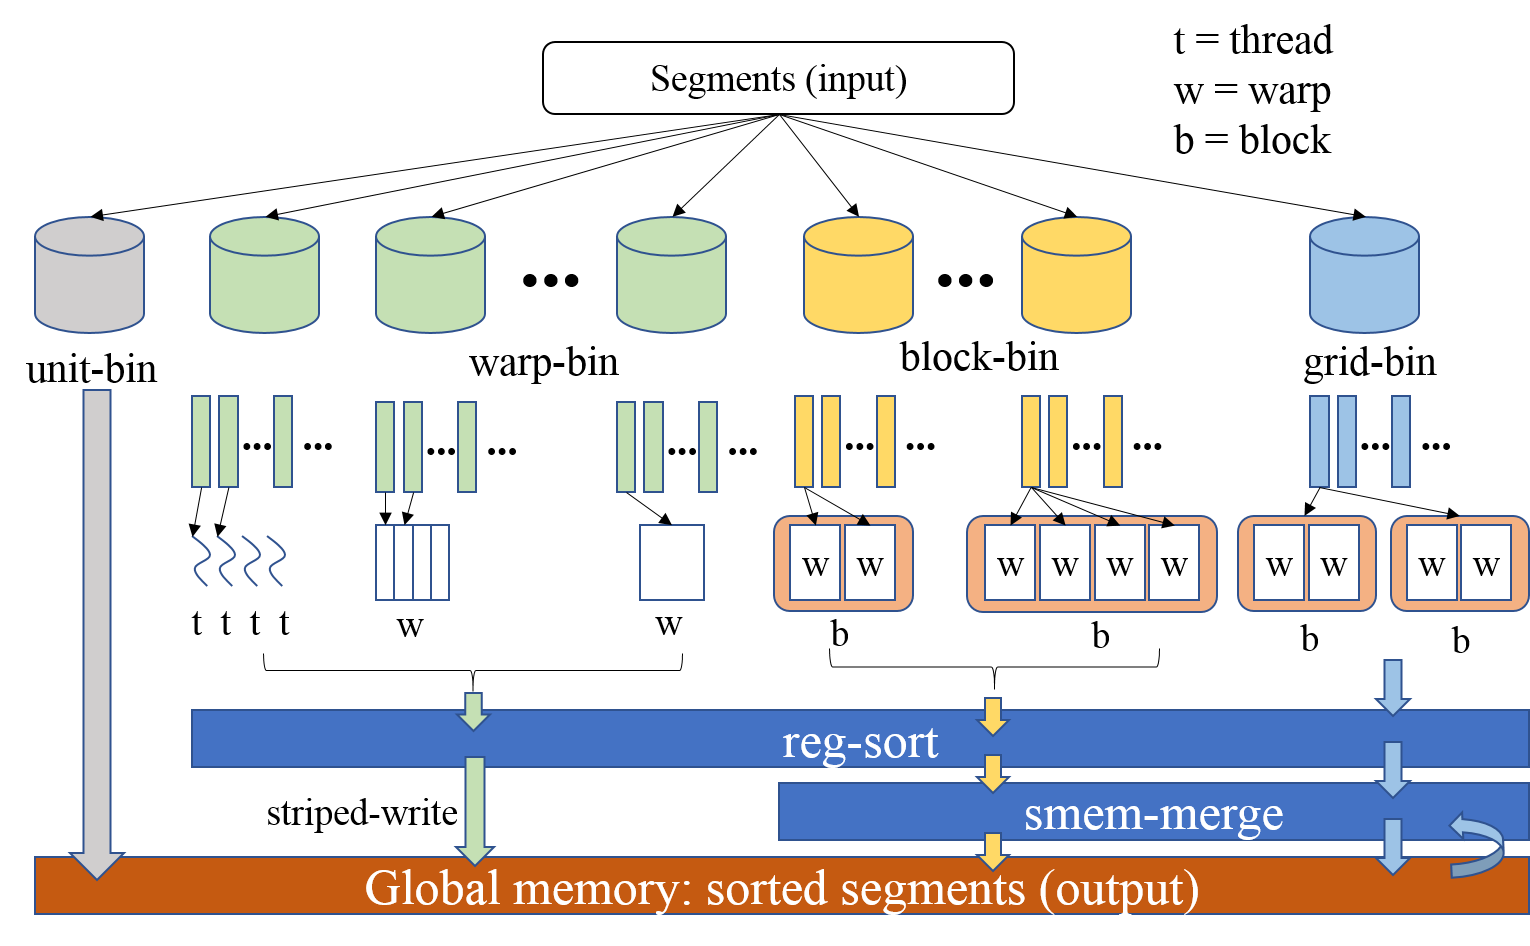
\includegraphics[scale=0.4]{image/fig_4_1.png}
    \caption{Overview of fast segmented sort}
    \label{fig:fig_4_1}
\end{figure}

% avoid atomic
\subsection{Reducing atomic instruction}
In counting range phase, change the implementation similar as the mapping range phase in multi-slab version, now each thread handles one slab instead of one rectangle. This way can avoid to use atomic instruction, which breaks performance when using frequently, to speed up the computing time.

% load balance
\subsection{Load balance}
The task of checking the rectangles is imbalance. The 32rd thread needs to run 31 times and first thread no needs to do anything. We use shuffle instruction to make it load balance, and it can avoid to synchronize threads or access violate shared memory which the latency is higher than register operation. Fig. \ref{fig:fig_4_3} shows the steps of using shuffle to make the task be load balance.
\begin{figure}[h]
    \centering
    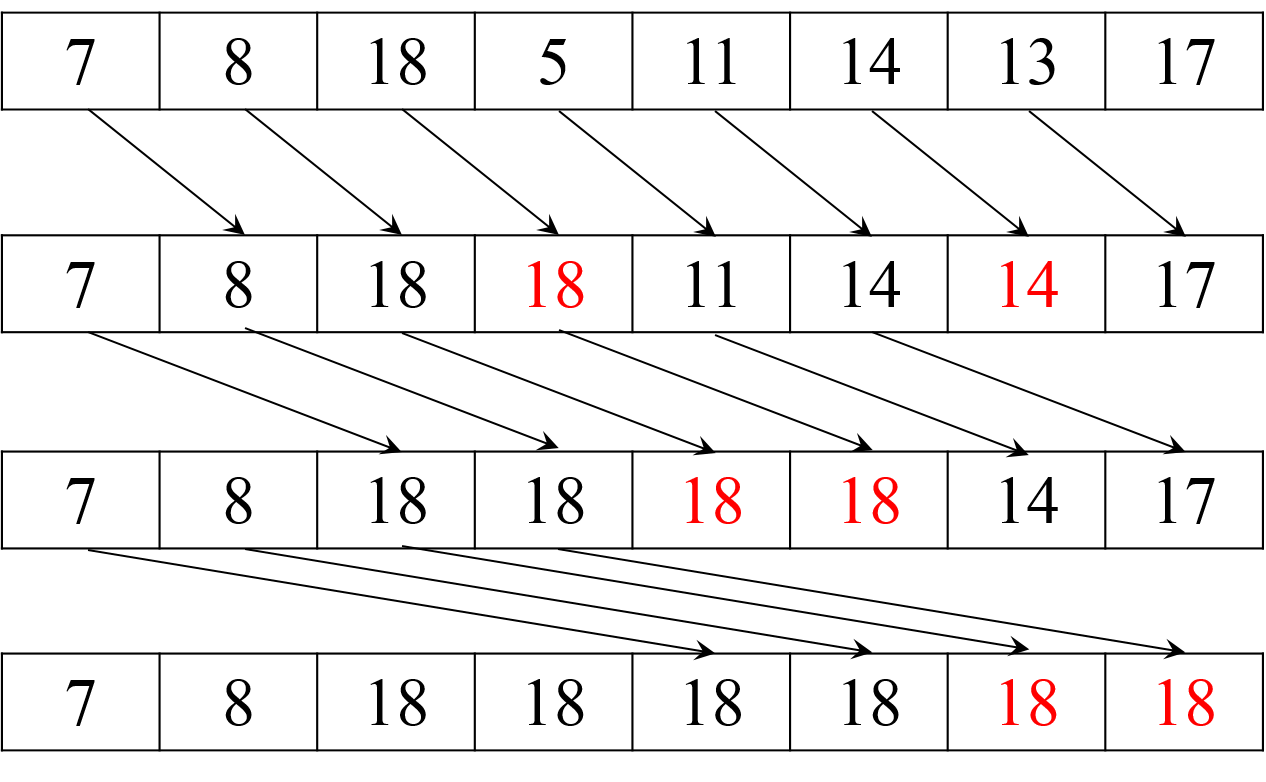
\includegraphics[scale=0.4]{image/fig_4_3.png}
    \caption{Example of load balance in parallel prefix max using shfl\_up instruction }
    \label{fig:fig_4_3}
\end{figure}

%%%%%%%%%%%%%%%%%%%%%%%%%%%%%%%%%%%%%%%%%%%%%%%%55
\section{Calculating right triangle union area in CPU}
In our GPU implementations, we only deal with rectangles and do not consider right triangles. In order to fully use computing resource, we calculate right triangles using CPU. First, we decompose vertical trapezoids into one rectangle and two right triangles, and deal with them as three rectangles on GPU because we want to use \textit{rectangle array} to map window faster and reduce computing time. We add a flag to identify the object which is rectangle or one of the four types of right triangles. Then, each triangle is computed union area as rectangle on GPU, so we need to subtract the difference area of the triangle. For this purpose, we scan all triangle in each window, and use line sweep algorithm to obtain the difference area which is not covered by other objects in this window.

\subsection{Finding out intersection points}
It is not necessary to find out the intersection points with all objects in this window, we only need to consider the object which is intersection with the triangle's boundary (to simplify the calculation, we use rectangle's boundary to represent the triangle). We classify edges into two categories, horizontal and hypotenuse, to reduce the computing task.  If the line is belong to horizontal, it only need to find intersection points with lines which are belong to hypotenuse. We sort the intersection points and x axis value of each object after we find out all intersection points.

\subsection{Calculating area}
In this step, we need to calculate this triangle's area which is not covered by other rectangles and triangles. We compute the total area in each slab at first, and using line sweep algorithm to calculate the union area and subtract it to the total area. We also check the window's boundary. Finally, we can obtain the value which is needed to subtract the result from GPU.

In order to deal with the union area between triangles, we make the triangle as rectangle after we already calculate its area. (see Fig. \ref{fig:fig_3_7})

\begin{figure}[h]
    \centering
    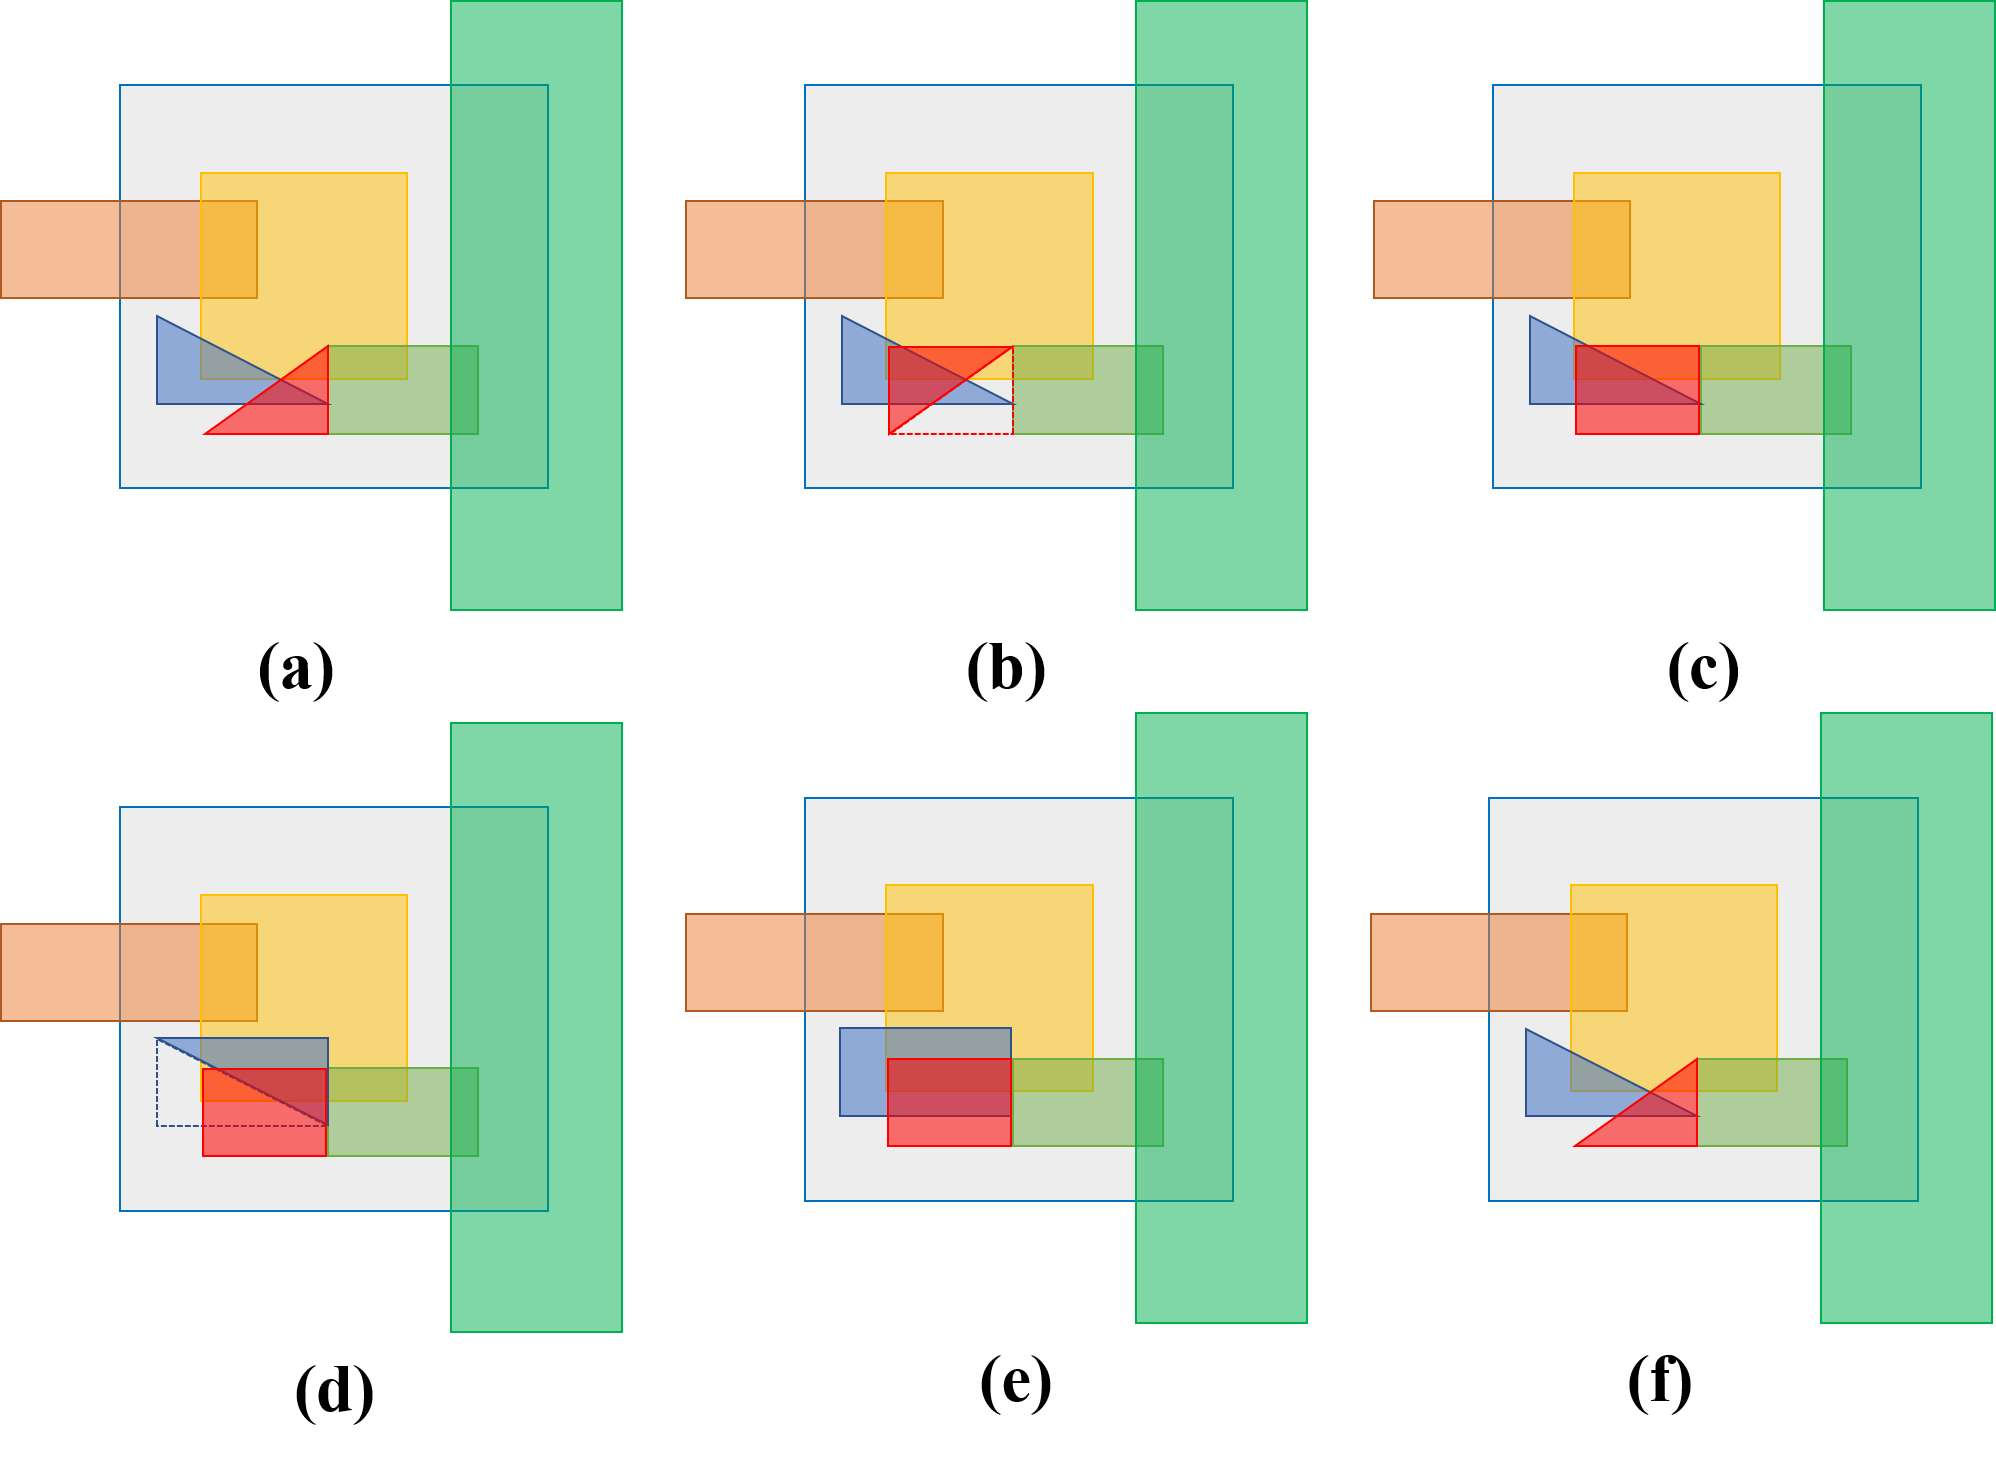
\includegraphics[scale=0.4]{image/fig_3_7}
    \caption{(a) origin input data in the window
(b) calculating the difference area of red triangle 
(c) treat red triangle as rectangle after computing its difference area
(d) calculating the difference area of blue triangle
(e) treat blue triangle as rectangle after computing its difference area 
(f) the input data does not change
}
    \label{fig:fig_3_7}
\end{figure}
%\chapter{Optimization}
\label{chap:optimizations}



\chapter{Experiments}
\label{chap:experiments}
This chapter presents the results of eight sets of experiments for the implementation. The first experiment profiles the execution time of each phase on GPU. The second experiment focus on each optimization techniques. The third experiment compares the performance of CPU and GPU version. The fourth experiment shows the scalability of our implementation. The fifth and the sixth experiments compares the different testcases with different degree of coverage of rectangles and proportion of right triangles respectively. The seventh experiment investigates the results for different setting in checking memeory for windows (group). The eighth experiment discusses the sampling method to estimate the value of $\beta$.

The CPU used in the experiments is Intel Core i7-5820K, and the GPU is GeForce GTX 750 Ti with 4 GB global memory and its compute capability is 5.0. Each block has 48 KB shared memory and 65536 32 bits registers. We also use the GeForce GTX 1080 Ti with 11 GB global memory and its compute capabibity is 6.1. Each block has 96 KB shared memory and 65536 32 bits registers. We use two testcase in the experiment, their cell’s boundary is (0, 0) to (4700000, 4500000) and the number of total rectangles is both ten million. The lengths of rectangles are both one thousand in testcase 1. Contrary with it, the lengths of rectangles in testcase 2 are from one hundred to twenty thousand one hundred. the difference between two testcase is degree of coverage.

\section{Computing time of each phase}
From table \ref{table:5_1} to table \ref{table:5_8} show the profiles of the computing time on GPU for testcase 1 and testcase 2 respectively. The values in brackets which connected after the testcase are window size and window stride respectively. Multi-sweep-line (MSL) version is multi-slab version with all optimizations we described before. To focus on our implementations, all our three versions use fast segmented sort.

\begin{table}[!h]
\centering
\newcommand{\tabincell}[2]{\begin{tabular}{@{}#1@{}}#2\end{tabular}}
\begin{tabular}{| l | c | c | c | c | c | c | c | c |} 
 \hline
  & sampling & counting & mapping & sorting & \tabincell{c}{counting\\range} & \tabincell{c}{mapping\\range} & computing & total\\ [0.5ex] \hline
  baseline &  & 108 & 105 & 41 &  &  & 3,639 & 3,893\\ \hline
  multi-slab & 777 & 112 & 114 & 101 & 310 & 275 & 836 & 2,525\\ \hline
  MSL & 778 & 112 & 114 & 101 & 230 & 410 & 199 & 1,944\\ \hline
\end{tabular}
\caption{The computing time of each phase for testcase1(10000, 10000) on GTX 750 Ti(unit: ms)}
\label{table:5_1}
\end{table}

\begin{table}[!h]
\centering
\newcommand{\tabincell}[2]{\begin{tabular}{@{}#1@{}}#2\end{tabular}}
\begin{tabular}{| l | c | c | c | c | c | c | c | c |} 
 \hline
  & sampling & counting & mapping & sorting & \tabincell{c}{counting\\range} & \tabincell{c}{mapping\\range} & computing & total\\ [0.5ex] \hline
  baseline &  & 208 & 215 & 151 &  &  & 14,423 & 14,997\\ \hline
  multi-slab & 777 & 225 & 231 & 389 & 1,281 & 1,020 & 3,302 & 7,225\\ \hline
  MSL & 778 & 223 & 231 & 390 & 861 & 1,636 & 805 & 4,924\\ \hline
\end{tabular}
\caption{The computing time of each phase for testcase1(10000, 5000) on GTX 750 Ti(unit: ms)}
\label{table:5_2}
\end{table}

\begin{table}[!h]
\centering
\newcommand{\tabincell}[2]{\begin{tabular}{@{}#1@{}}#2\end{tabular}}
\begin{tabular}{| l | c | c | c | c | c | c | c | c |} 
 \hline
  & sampling & counting & mapping & sorting & \tabincell{c}{counting\\range} & \tabincell{c}{mapping\\range} & computing & total\\ [0.5ex] \hline
  baseline &  & 139 & 144 & 158 &  &  & 21,631 & 22,072\\ \hline
  multi-slab & 777 & 143 & 156 & 299 & 1,813 & 1,599 & 2,272 & 7,059\\ \hline
  MSL & 775 & 142 & 158 & 300 & 567 & 1,187 & 1,391 & 4,520\\ \hline
\end{tabular}
\caption{The computing time of each phase for testcase2(10000, 10000) on GTX 750 Ti (unit: ms)}
\label{table:5_3}
\end{table}

\begin{table}[!h]
\centering
\newcommand{\tabincell}[2]{\begin{tabular}{@{}#1@{}}#2\end{tabular}}
\begin{tabular}{| l | c | c | c | c | c | c | c | c |} 
 \hline
  & sampling & counting & mapping & sorting & \tabincell{c}{counting\\range} & \tabincell{c}{mapping\\range} & computing & total\\ [0.5ex] \hline
  baseline &  & 281 & 371 & 619 &  &  & 89,469 & 90,740\\ \hline
  multi-slab & 777 & 292 & 391 & 1,183 & 7,255 & 6,593 & 8,856 & 25,347\\ \hline
  MSL & 776 & 293 & 391 & 1,184 & 2,303 & 4,751 & 5,542 & 15,240\\ \hline
\end{tabular}
\caption{The computing time of each phase for testcase2(10000, 5000) on GTX 750 Ti (unit: ms)}
\label{table:5_4}
\end{table}

\begin{table}[!h]
\centering
\newcommand{\tabincell}[2]{\begin{tabular}{@{}#1@{}}#2\end{tabular}}
\begin{tabular}{| l | c | c | c | c | c | c | c | c |} 
 \hline
  & sampling & counting & mapping & sorting & \tabincell{c}{counting\\range} & \tabincell{c}{mapping\\range} & computing & total\\ [0.5ex] \hline
  baseline &  & 11 & 12 & 17 &  &  & 583 & 623\\ \hline
  multi-slab & 82 & 10 & 10 & 31 & 44 & 46 & 102 & 325\\ \hline
  MSL & 81 & 9 & 10 & 27 & 34 & 36 & 25 & 222\\ \hline
\end{tabular}
\caption{The computing time of each phase for testcase1(10000, 10000) on GTX 1080 Ti(unit: ms)}
\label{table:5_5}
\end{table}

\begin{table}[!h]
\centering
\newcommand{\tabincell}[2]{\begin{tabular}{@{}#1@{}}#2\end{tabular}}
\begin{tabular}{| l | c | c | c | c | c | c | c | c |} 
 \hline
  & sampling & counting & mapping & sorting & \tabincell{c}{counting\\range} & \tabincell{c}{mapping\\range} & computing & total\\ [0.5ex] \hline
  baseline &  & 21 & 24 & 63 &  &  & 2,068 & 2,176\\ \hline
  multi-slab & 83 & 20 & 23 & 113 & 167 & 169 & 400 & 975\\ \hline
  MSL & 81 & 18 & 21 & 114 & 114 & 145 & 95 & 588\\ \hline
\end{tabular}
\caption{The computing time of each phase for testcase1(10000, 5000) on GTX 1080 Ti(unit: ms)}
\label{table:5_6}
\end{table}

\begin{table}[!h]
\centering
\newcommand{\tabincell}[2]{\begin{tabular}{@{}#1@{}}#2\end{tabular}}
\begin{tabular}{| l | c | c | c | c | c | c | c | c |} 
 \hline
  & sampling & counting & mapping & sorting & \tabincell{c}{counting\\range} & \tabincell{c}{mapping\\range} & computing & total\\ [0.5ex] \hline
  baseline &  & 14 & 18 & 56 &  &  & 3,274 & 3,362\\ \hline
  multi-slab & 85 & 13 & 16 & 74 & 158 & 1,678 & 767 & 2,791\\ \hline
  MSL & 81 & 13 & 16 & 81 & 77 & 99 & 238 & 605\\ \hline
\end{tabular}
\caption{The computing time of each phase for testcase2(10000, 10000) on GTX 1080 Ti (unit: ms)}
\label{table:5_7}
\end{table}

\begin{table}[!h]
\centering
\newcommand{\tabincell}[2]{\begin{tabular}{@{}#1@{}}#2\end{tabular}}
\begin{tabular}{| l | c | c | c | c | c | c | c | c |} 
 \hline
  & sampling & counting & mapping & sorting & \tabincell{c}{counting\\range} & \tabincell{c}{mapping\\range} & computing & total\\ [0.5ex] \hline
  baseline &  & 30 & 48 & 193 &  &  & 12,848 & 13,119\\ \hline
  multi-slab & 83 & 27 & 47 & 294 & 616 & 6,645 & 2,928 & 10,640\\ \hline
  MSL & 75 & 23 & 41 & 291 & 281 & 395 & 999 & 2,105\\ \hline
\end{tabular}
\caption{The computing time of each phase for testcase2(10000, 5000) on GTX 1080 Ti (unit: ms)}
\label{table:5_8}
\end{table}

Comparing tables \ref{table:5_1} and \ref{table:5_3}, which are using different testcase, one can find that computing time after sorting step is increased. The reason for this condition is because of the degree of overlap is more serious in testcase 2. The computing time before sorting step almost nothing changes because the total number of rectangles is same between two testcases.

\section{Optimization techniques}

\subsection{Fast segmented sort}
Table \ref{table:5_9} and table \ref{table:5_10} show the sorting performance of using fast segmented sort. It is almost 9 $\sim$ 90 times faster than origin sorting, which we using thrust in kernel function.
\begin{table}[h!]
\centering
\begin{tabular}{| l | c | c |} 
 \hline
  & Thrust sort & Fast segmented sort \\ [0.5ex] \hline
  Testcase 1 (10000, 10000) & 922 & 101\\ \hline
  Testcase 1 (10000, 5000) & 3,456 & 390\\ \hline
  Testcase 2 (10000, 10000) & 2,880 & 300\\ \hline
  Testcase 2 (10000, 5000) & 8,013 & 1,184\\ \hline
\end{tabular}
\caption{The computing time of sorting on GTX 750 Ti (unit: ms)}
\label{table:5_9}
\end{table}

\begin{table}[h!]
\centering
\begin{tabular}{| l | c | c |} 
 \hline
  & Thrust sort & Fast segmented sort \\ [0.5ex] \hline
  Testcase 1 (10000, 10000) & 2,567 & 27\\ \hline
  Testcase 1 (10000, 5000) & 6,625 & 114\\ \hline
  Testcase 2 (10000, 10000) & 7,365 & 81\\ \hline
  Testcase 2 (10000, 5000) & 12,319 & 291\\ \hline
\end{tabular}
\caption{The computing time of sorting on GTX 1080 Ti (unit: ms)}
\label{table:5_10}
\end{table}

\subsection{Reducing atomic instruction}
Table \ref{table:5_11} and table \ref{table:5_12} show the difference of reducing atomic instruction in counting range phase. It can speedup 1.2 $\sim$ 3 times in testcase 1 and testcase 2.
\begin{table}[!h]
\centering
\begin{tabular}{| l | c | c |} 
 \hline
  & With atomic instruction & Without atomic instruction \\ [0.5ex] \hline
  Testcase 1 (10000, 10000) & 311 & 230\\ \hline
  Testcase 1 (10000, 5000) & 1,211 & 861\\ \hline
  Testcase 2 (10000, 10000) & 1,817 & 567\\ \hline
  Testcase 2 (10000, 5000) & 7,358 & 2,303\\ \hline
\end{tabular}
\caption{The computing time of counting range phase on GTX 750 Ti (unit: ms)}
\label{table:5_11}
\end{table}

\begin{table}[!h]
\centering
\begin{tabular}{| l | c | c |} 
 \hline
  & With atomic instruction & Without atomic instruction \\ [0.5ex] \hline
  Testcase 1 (10000, 10000) & 43 & 34\\ \hline
  Testcase 1 (10000, 5000) & 166 & 114\\ \hline
  Testcase 2 (10000, 10000) & 157 & 77\\ \hline
  Testcase 2 (10000, 5000) & 627 & 281\\ \hline
\end{tabular}
\caption{The computing time of counting range phase on GTX 1080 Ti (unit: ms)}
\label{table:5_12}
\end{table}

\subsection{Multi-sweep-line algorithm with load balance}
Table \ref{table:5_13} and table \ref{table:5_14} show the performance of using multi-sweep-line algorithm and load balance we presented in this thesis. It can improve computing phase approximate 1.6 $\sin$ 4 times in testcase 1 and testcase 2.
\begin{table}[!h]
\centering
\begin{tabular}{| l | c | c | c |} 
 \hline
  & Origin  & Multi-sweep-line without load balance & Multi-sweep-line \\ [0.5ex] \hline
  Testcase 1 (10000, 10000) & 835 & 255 & 199\\ \hline
  Testcase 1 (10000, 5000) & 3,279 & 1,017 & 804\\ \hline
  Testcase 2 (10000, 10000) & 2,270 & 1,749 & 1,391\\ \hline
  Testcase 2 (10000, 5000) & 8,917 & 6,980 & 5,542\\ \hline
\end{tabular}
\caption{The computing time of computing phase on GTX 750 Ti (unit: ms)}
\label{table:5_13}
\end{table}

\begin{table}[!h]
\centering
\begin{tabular}{| l | c | c | c |} 
 \hline
  & Origin  & Multi-sweep-line without load balance & Multi-sweep-line \\ [0.5ex] \hline
  Testcase 1 (10000, 10000) & 102 & 31 & 25\\ \hline
  Testcase 1 (10000, 5000) & 407 & 122 & 95\\ \hline
  Testcase 2 (10000, 10000) & 770 & 314 & 238\\ \hline
  Testcase 2 (10000, 5000) & 2,927 & 1,283 & 999\\ \hline
\end{tabular}
\caption{The computing time of computing phase on GTX 1080 Ti (unit: ms)}
\label{table:5_14}
\end{table}

\section{Comparison between GPU and CPU}
Fig. \ref{fig:fig_5_1}, Fig. \ref{fig:fig_5_2}, Fig. \ref{fig:fig_5_3}, and Fig. \ref{fig:fig_5_4} show the computing time of CPU and GPU version. The sequence CPU versions we used are provided by AnaGlobe Technology, Inc. They have two implementations. The first one is to compute general polygon union area, like boost geometry, it overlay all polygons and generate several new polygons, and then compute their area. The second one is optimized to calculate density (union), it decompose all non-rectilinear polygons into vertical trapezoids, and merge overlapped vertical trapezoids into non-overlapped vertical trapezoids, finally it can be easily to calculate vertical trapezoids area. We also tried to transform our GPU version algorithm to sequence code, but it is slower than the code provided by AnaGlobe Technology, Inc. For this reason, we only compare our implementation with their sequence codes. We do not show profile information because we cannot profile detail of their implementations. From Fig. \ref{fig:fig_5_1} to Fig. \ref{fig:fig_5_4} show that the total computing time of GPU versions is faster than CPU version and (10000, 10000) means the length of windows and the stride of each windows are both ten thousand. MSL speedup more than 20 and  77 times than sequence code on GTX 750 Ti and GTX 1080 Ti. It should be noted that the sampling time is same in multi-slab version and MSL version with different window setting, so the speedup in (10000, 10000) setting is not more obvious than (10000, 5000) due to the total computing time is smaller.

\begin{figure}[h]
    \centering
    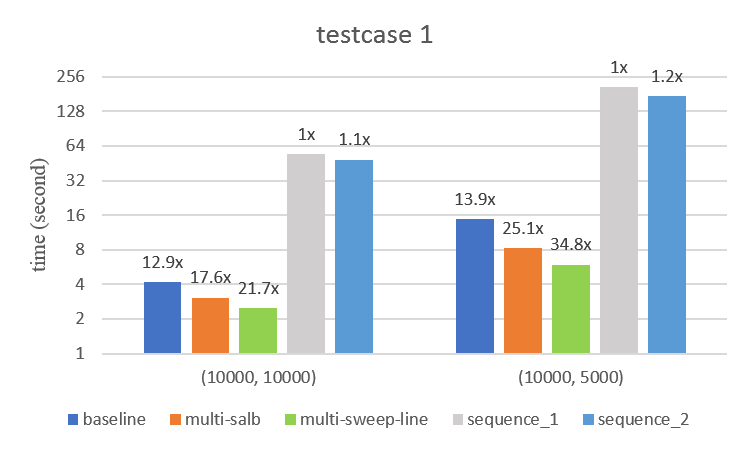
\includegraphics[scale=0.7]{image/fig_5_1}
    \caption{The computing time of CPU and GPU version in testcase 1 on GTX 750 Ti}
    \label{fig:fig_5_1}
\end{figure}

\begin{figure}[h]
    \centering
    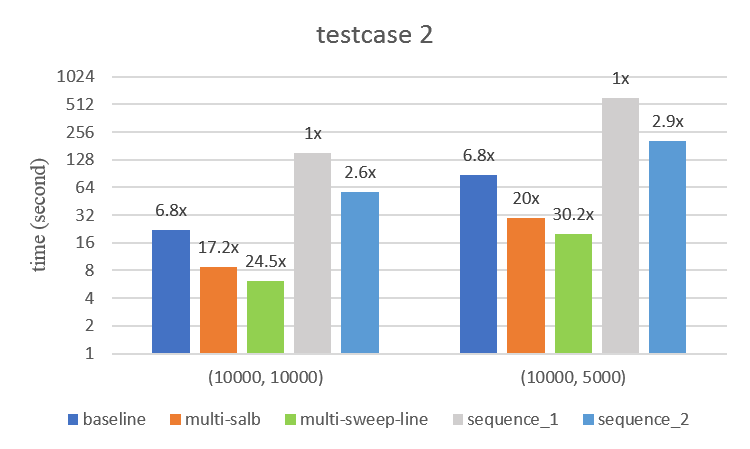
\includegraphics[scale=0.7]{image/fig_5_2}
    \caption{The computing time of CPU and GPU version in testcase 2 on GTX 750 Ti}
    \label{fig:fig_5_2}
\end{figure}

\begin{figure}[h]
    \centering
    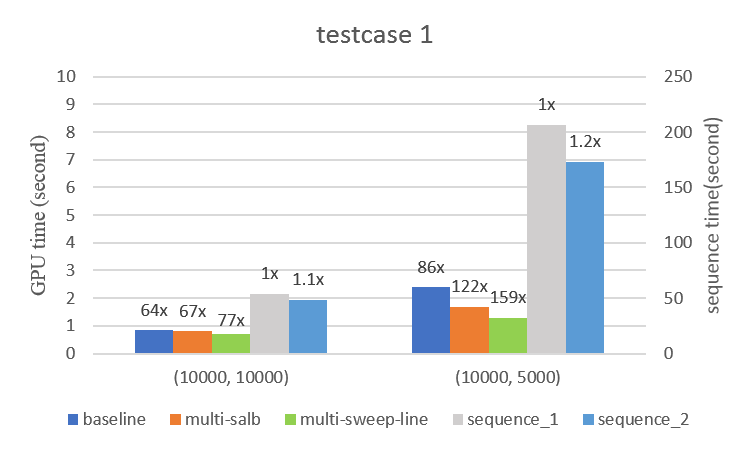
\includegraphics[scale=0.7]{image/fig_5_3}
    \caption{The computing time of CPU and GPU version in testcase 1 on GTX 1080 Ti}
    \label{fig:fig_5_3}
\end{figure}

\begin{figure}[h]
    \centering
    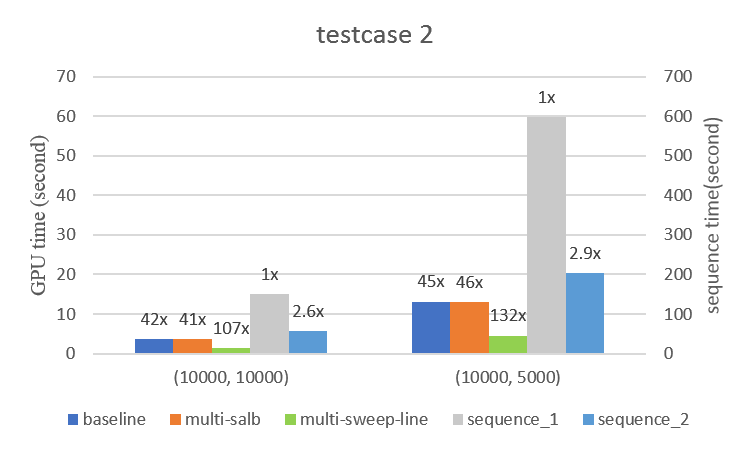
\includegraphics[scale=0.7]{image/fig_5_4}
    \caption{The computing time of CPU and GPU version in testcase 2 on GTX 1080 Ti}
    \label{fig:fig_5_4}
\end{figure}

\section{Multiple GPUs (scalability)}
Fig. \ref{fig:fig_5_5} and Fig. \ref{fig:fig_5_6} show the scalability of using multiple GPUs. We use K80 from one to four on one device node in the cluster. We only calculate the execution time except the time of rectangle information copy from host to device because the communication time between host node and device node is slower than computing time in GPUs.

\begin{figure}[h]
    \centering
    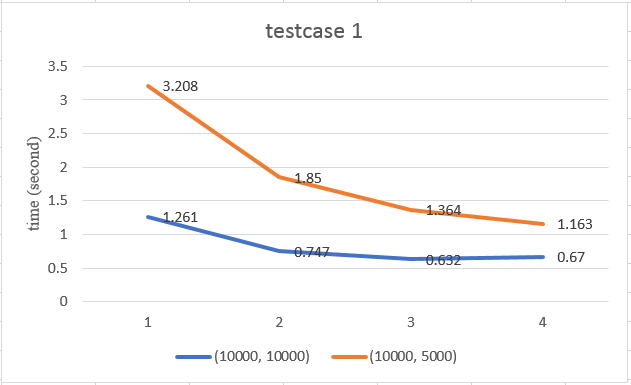
\includegraphics[scale=0.7]{image/fig_5_5}
    \caption{The strong scalability of Multi-sweep-line in testcase 1}
    \label{fig:fig_5_5}
\end{figure}

\begin{figure}[h]
    \centering
    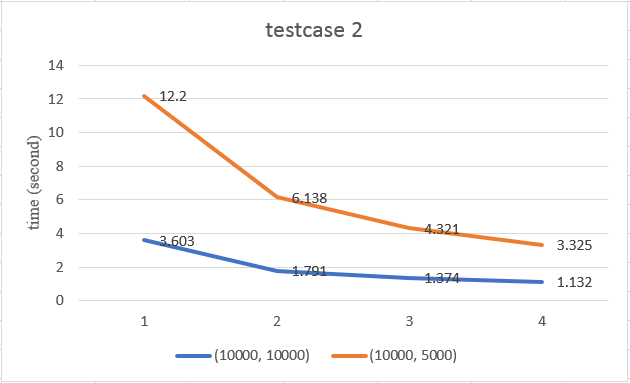
\includegraphics[scale=0.7]{image/fig_5_6}
    \caption{The strong scalability of Multi-sweep-line in testcase 2}
    \label{fig:fig_5_6}
\end{figure}

Our process uses less time when we using more GPUs, it provides strong scalability. The execution time between using 3 and 4 GPUs is similar when window size equals to window stride (blue line) in testcase 1 because the degree of coverage is not uniform and we equally partition the cell.

\section{Comparison between testcases with different degree of coverage}
From Fig. \ref{fig:fig_5_7} to Fig. \ref{fig:fig_5_10} show the comparison between testcases with different degree of coverage. When win\_stride is equal to 10000, the speedup is only 20 times and 70 times in GTX 750 Ti and GTX 1080 Ti. And the speedup is 30 times and 120 times in GTX 750 Ti and GTX 1080 Ti when win\_stride is equal to 5000. The reason for this condition is that the computing time of allocate and sampling are constant.

\begin{figure}[!h]
    \centering
    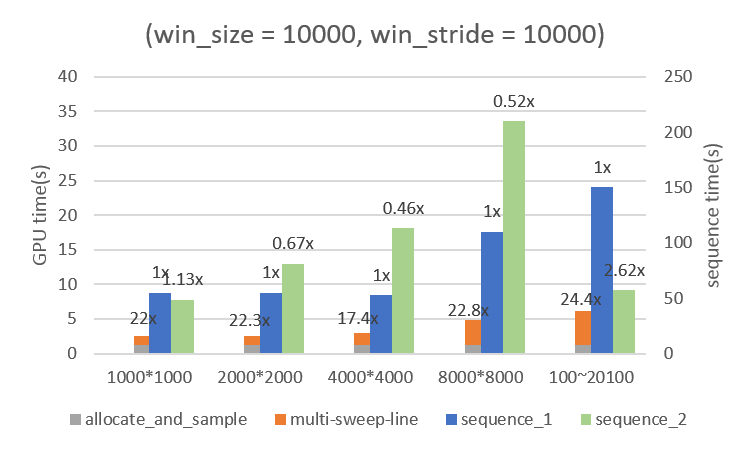
\includegraphics[scale=0.7]{image/fig_5_7}
    \caption{The computing time of multi-sweep-line and sequences in testcases with different degree of coverage (win\_size = 10000, win\_stride = 10000) on GTX 750 Ti}
    \label{fig:fig_5_7}
\end{figure}

\begin{figure}[!h]
    \centering
    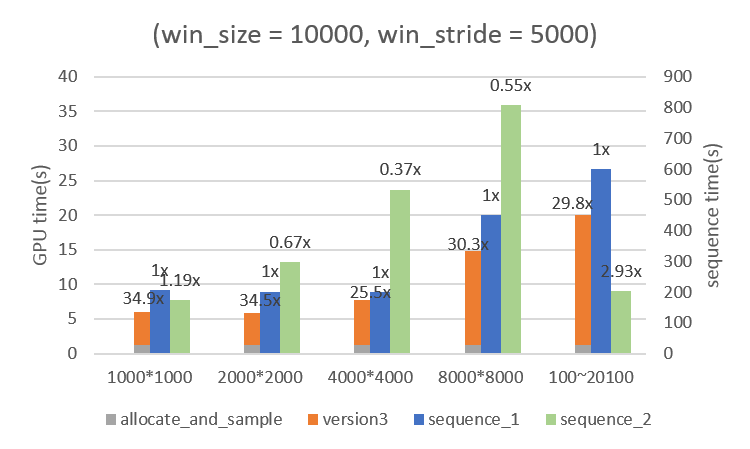
\includegraphics[scale=0.7]{image/fig_5_8}
    \caption{The computing time of multi-sweep-line and sequences in testcases with different degree of coverage (win\_size = 10000, win\_stride = 5000) on GTX 750 Ti}
    \label{fig:fig_5_8}
\end{figure}

\begin{figure}[!h]
    \centering
    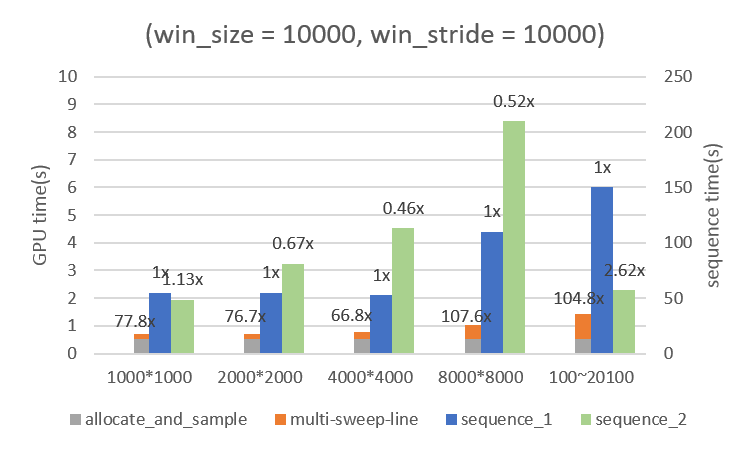
\includegraphics[scale=0.7]{image/fig_5_9}
    \caption{The computing time of multi-sweep-line and sequences in testcases with different degree of coverage (win\_size = 10000, win\_stride = 10000) on GTX 1080 Ti}
    \label{fig:fig_5_9}
\end{figure}

\begin{figure}[!h]
    \centering
    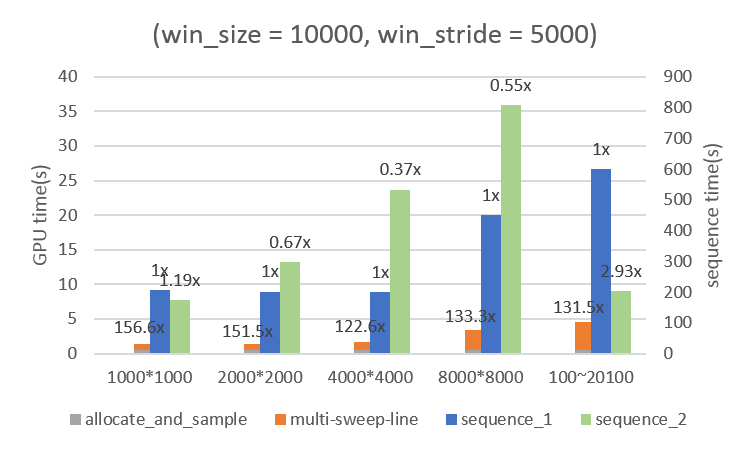
\includegraphics[scale=0.7]{image/fig_5_10}
    \caption{The computing time of multi-sweep-line and sequences in testcases with different degree of coverage (win\_size = 10000, win\_stride = 5000) on GTX 1080 Ti}
    \label{fig:fig_5_10}
\end{figure}

\section{Comparison between testcases with different proportion of right triangles}
From Fig. \ref{fig:fig_5_11} to Fig. \ref{fig:fig_5_14} show the comparison between testcases with different proportion of triangles. If we use OpenMP to accelerate the calculating time of triangles on CPU, it can be almost completely overlapping in the computing time on GPU.

\begin{figure}[!h]
    \centering
    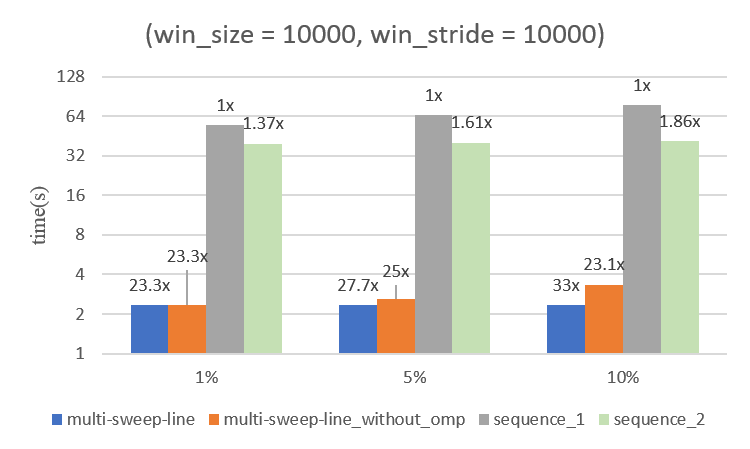
\includegraphics[scale=0.7]{image/fig_5_11}
    \caption{The computing time of multi-sweep-line, multi-sweep-line without OpenMP and sequences in testcases with different proportion of triangles (win\_size = 10000, win\_stride = 10000) on GTX 750 Ti}
    \label{fig:fig_5_11}
\end{figure}

\begin{figure}[!h]
    \centering
    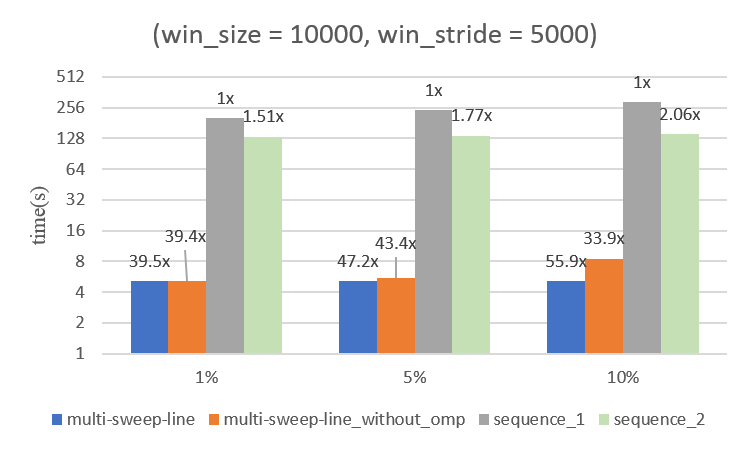
\includegraphics[scale=0.7]{image/fig_5_12}
    \caption{The computing time of multi-sweep-line, multi-sweep-line without OpenMP and sequences in testcases with different proportion of triangles (win\_size = 10000, win\_stride = 5000) on GTX 750 Ti}
    \label{fig:fig_5_12}
\end{figure}

\begin{figure}[!h]
    \centering
    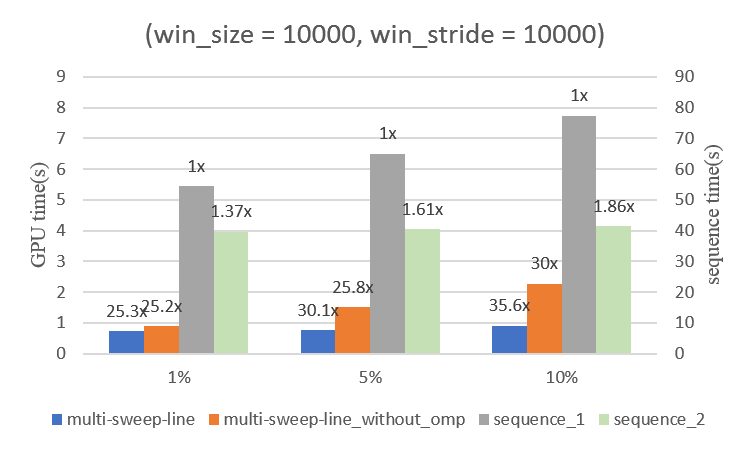
\includegraphics[scale=0.7]{image/fig_5_13}
    \caption{The computing time of multi-sweep-line, multi-sweep-line without OpenMP and sequences in testcases with different proportion of triangles (win\_size = 10000, win\_stride = 10000) on GTX 1080 Ti}
    \label{fig:fig_5_13}
\end{figure}

\begin{figure}[!h]
    \centering
    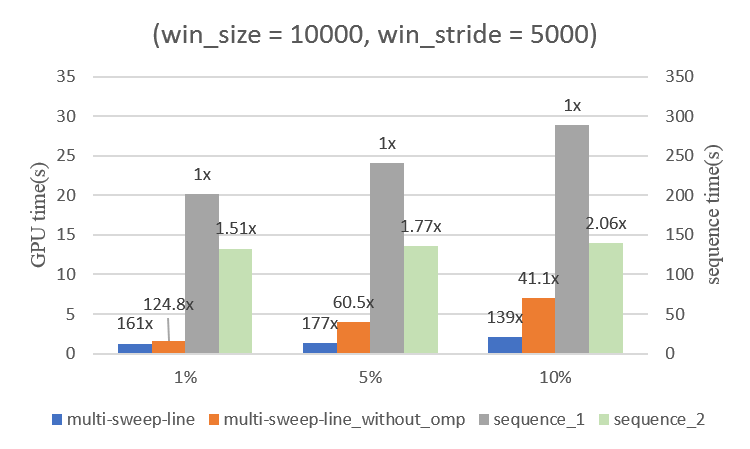
\includegraphics[scale=0.7]{image/fig_5_14}
    \caption{The computing time of multi-sweep-line, multi-sweep-line without OpenMP and sequences in testcases with different proportion of triangles (win\_size = 10000, win\_stride = 5000) on GTX 1080 Ti}
    \label{fig:fig_5_14}
\end{figure}

\section{Discussion for the checking memory for windows (group)}
Table \ref{table:5_15} shows the results for different setting in checking memory for windows. The total in table means the process checks total memory usage including additional array (\textit{range counter array}, \textit{range offset array}, and \textit{range rectangle array}) and partition task. The value 1/600 means the process does not consider whole these three arrays, it only checks other memory usage and these three arrays divided by 600. We can see that there is no significant differences on 1080 Ti, but it is slower on 750 Ti if the process checks whole memory usage. The reason for this situation is that three additional array is larger than global memory and it will make process partition the task into many subtask. The computing time of counting phase and mapping phase is increasing. So we choose 1/400 in our process according to the experiment.

\begin{table}[!h]
\centering
\begin{tabular}{|c|l|c|l|c|}
\hline
\multicolumn{1}{|l|}{}   & \multicolumn{2}{l|}{testcase 1 (10000, 5000)} & \multicolumn{2}{l|}{testcase 2 (10000, 5000)} \\ \hline
\multirow{6}{*}{750 Ti}  & total & 7.202732 & total & 33.134935 \\ \cline{2-5} 
                         & 1/600 & 5.92086 & 1/600 & 20.283393 \\ \cline{2-5} 
                         & 1/500 & 5.929029 & 1/500 & 20.047735 \\ \cline{2-5} 
                         & 1/400 & 5.928557 & 1/400 & 20.040704 \\ \cline{2-5} 
                         & 1/300 & 5.92923 & 1/300 & 21.20294 \\ \cline{2-5} 
                         & 1/200 & 5.928677 & 1/200 & 21.364763 \\ \hline
\multirow{6}{*}{1080 Ti} & total & 1.416512 & total & 4.274711 \\ \cline{2-5} 
                         & 1/600 & 1.319576 & 1/600 & 4.527126 \\ \cline{2-5} 
                         & 1/500 & 1.315042 & 1/500 & 4.51068 \\ \cline{2-5} 
                         & 1/400 & 1.303876 & 1/400 & 4.567402 \\ \cline{2-5} 
                         & 1/300 & 1.307797 & 1/300 & 4.53494 \\ \cline{2-5} 
                         & 1/200 & 1.325864 & 1/200 & 4.505561 \\ \hline
\end{tabular}
\caption{The comparison results of checking memory for windows with different setting (unit: second)}
\label{table:5_15}
\end{table}

\section{Discussion for the sampling methods}
Table \ref{table:5_16} shows the results for different sampling method to estimate the number of rectangles in range rectangle array. Method 1 is using $\alpha$ to estimate the value of $\beta$ which we present in section 3.3.4; Method 2 is sampling to obtain not only $\alpha$ but also $\beta$. The difference means difference between the value we estimate and the real value in each testcase. Method 1 uses less time and small difference in testcase 2. The discrepancy between method 1 and method 2 in testcase 1 is similar (not consider positive or negative). We prefer to estimate larger number if difference is same, because we do not want to partition the task in next checking memory phase. Fig. \ref{fig:fig_5_15} shows the computing time of testcase 2 (win\_size = 10000, win\_stride = 5000) on GPU 750 Ti.

It should be noted that the process does not use $\beta$ in testcase 1 on GPU 750 Ti because the memory usage of testcase 1 is smaller than testcase 2.

\begin{table}[h!]
\centering
\begin{tabular}{| l | c | c | c |} 
 \hline
  & Method 1 (difference) & Method 2 (difference) & Real \\ [0.5ex] \hline
  Testcase 1 (10000, 10000) & 352,937,165 (65\%) & 81,626,040 (-61.68\%) & 213,021,830\\ \hline
  Testcase 1 (10000, 5000) & 1,414,292,101 (66.4\%) & 287,502,262 (-66.17\%) & 849,893,958\\ \hline
  Testcase 2 (10000, 10000) & 3,759,366,934 (-0.43\%) & 3,443,852,187 (-8.79\%) & 3,775,973,474\\ \hline
  Testcase 2 (10000, 5000) & 15,035,545,349 (-0.42\%) & 13,798,415,684 (-8.61\%) & 15,099,020,249\\ \hline
\end{tabular}
\caption{The comparison results of sampling methods (unit: rectangle)}
\label{table:5_16}
\end{table}

\begin{figure}[!h]
    \centering
    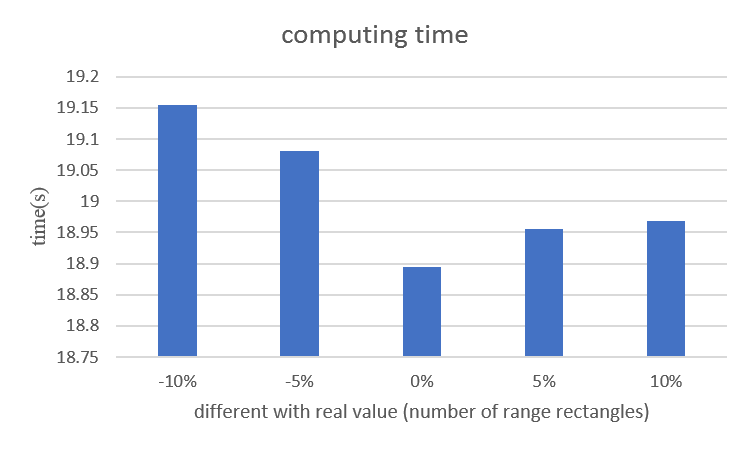
\includegraphics[scale=0.7]{image/fig_5_15}
    \caption{The computing time of different percentage with real value of range rectangle array (unit: rectangles)}
    \label{fig:fig_5_15}
\end{figure}
\chapter{Conclusion}
\label{chap:conclusion}
In this thesis, we have implemented the process, which is to calculate the density of rectangles and right triangles in the cell through GPU and CPU. And we have presented an adaptive task partition method and multi-sweep-line algorithm, which is more suitable for GPU architecture. Optimization techniques, including fast segmented sort, reducing atomic instruction, load balance ,are also applied to further improve the performance. The GPU implementation are accelerated approximately 75 $\sim$ 160 times than sequence CPU version on GTX 1080 Ti and it can be easily extended to multiple GPUs.

In the future, we would like to extend this method to support with more general polygon to handle more general purpose applications.


\bibliographystyle{plain}
\bibliography{note}

% The following two commands are all you need in the
% initial runs of your .tex file to
% produce the bibliography for the citations in your paper.
%{%\scriptsize
%\bibliographystyle{abbrv}
%\bibliography{HPCoC_cite}
%}
% You must have a proper ".bib" file
%  and remember to run:
% latex bibtex latex latex
% to resolve all references

\end{document}
